% Chapter 1

\chapter{Introduction} % Main chapter title

\label{Chapter1} % For referencing the chapter elsewhere, use \ref{Chapter1} 

%----------------------------------------------------------------------------------------

% Define some commands to keep the formatting separated from the content 
\newcommand{\keyword}[1]{\textbf{#1}}
\newcommand{\tabhead}[1]{\textbf{#1}}
\newcommand{\code}[1]{\texttt{#1}}
\newcommand{\file}[1]{\texttt{\bfseries#1}}
\newcommand{\option}[1]{\texttt{\itshape#1}}

%----------------------------------------------------------------------------------------

\section{Finding the correct representation}

A fundamental question in the cognitive sciences is how humans and
other organisms percieve complex stimuli, such as faces, objects, and
sounds.  A highly related question in artificial intelligence is how
to engineer systems that can learn how to identify objects, faces, and
parse the meaning of language.  Through the last couple of decades,
breakthroughs in both the understanding of cognition, and developments
in artificial intelligence, both suggest that \emph{nonlinear
  representations} are key for making sense of complex stimuli,
regardless of whether the perciever is a biological or algorithmic.

\subsection{Example: Receptive-field models for vision}

Let us begin with the biological case.  By looking at the neural
pathways involved in mammalian vision, neuroscientists know that
vision begins in the retina, where light-sensitive cells (rods and
cones) detect incoming photons.  The signals from the rods and cones
are aggregated by retinal cells, and then transmitted sequentially
through a series of structures within the brain--the dominant pathway
goes from the retina to the the optic chiasm, then to the lateral
geniculate nucleus, and finally to the visual cortex (Figure
\ref{fig:visual_pathway}).  The visual cortex, in turn, is divided
into subregions V1 through V6.  It is an active area of research to
study the specialized roles of each subregion with regards to visual
processing.

\begin{figure}
\centering
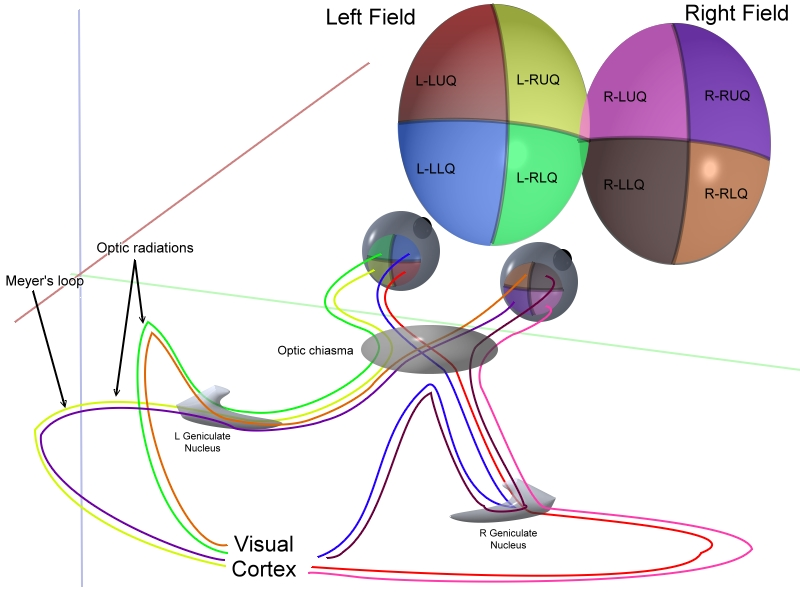
\includegraphics[scale = 1]{Figures/ERP_-_optic_cabling.jpg}
\caption{Visual pathway in humans.  Image credit to Ratznium under CC 2.5 license.}
\label{fig:visual_pathway}
\end{figure}

Functional MRI (fMRI) studies of vision provide one means of testing
theories about the workings of the visual cortex.  In an exemplary
study, \cite{Kay2008a} model the response of the BOLD fMRI signal (a
proxy measure of neural activity) to greyscale natural images
presented to a human subject.  The data takes the form of pairs
$(\vec{z}_i, \vec{y}_i)$, where $\vec{z}_i$ is the pixel intensities
of the presented image, and $\vec{y}_i$ is a three-dimensional map of
BOLD signal, represented as a numerical vector with one real-valued
intensity per voxel.

Kay et al. test two different models for the \emph{receptive field}
(RF) of V1 voxels.  A receptive field model, in this case, specifies a
specific set of transformations for explaining how visual information
is \emph{represented} in the V1 area of the brain.  Under one RF
model, the activity of V1 voxels can be explained by
\emph{retinotopic} receptive fields, in which the raw image
$\vec{z}_i$ is represented by a library of local luminance and
contrast maps.  Under the second RF model, the activity of V1 voxels
is explained by \emph{Gabor filter} receptive fields, consisting of
sinusoidal filters which are sensitive to position, frequency, and
orientation (Figure \ref{fig:gabor}).

\begin{figure}
\centering
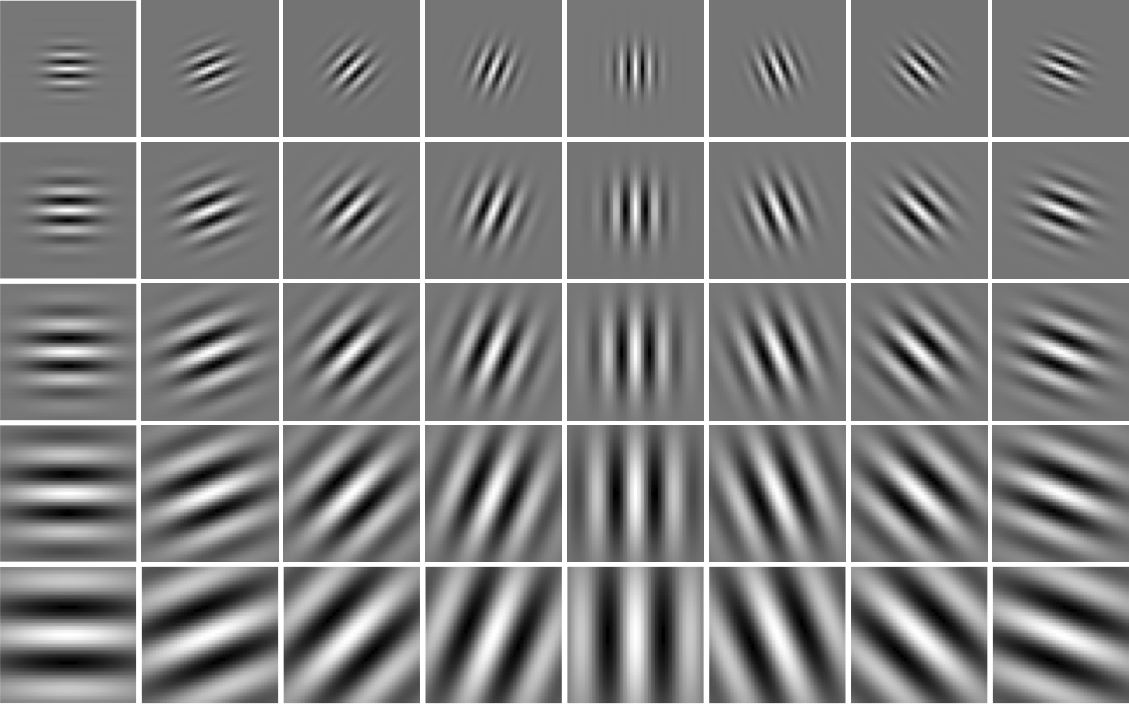
\includegraphics[scale = 0.5]{Figures/Gabor.jpg}
\caption{Examples of Gabor filters of varying size and orientation.  From \cite{haghighat2015cloudid}.}
\label{fig:gabor}
\end{figure}

Each receptive field model corresponds to a family
\emph{representations}, which is a family $\vec{g} = (g_1,\hdots,
g_m)$ of linear or nonlinear transformations of the visual stimulus
$\vec{z}$.  Let $z_j$ denote the intensity of the $j$th pixel in the
visual stimulus, and let $\ell_j = (r_j, c_j)$ indicate the row and
column coordinates of the $j$th pixel.  Under the retinotopic model,
the transformations consist of locally-weighted mean-luminance and
contrast operations,
\[
L(\vec{z}) = \frac{\sum_j w_j z_j}{\sum_j w_j}
\]
\[
C(\vec{z}) = \sqrt{\frac{\sum_j w_j (z_j - L(\vec{z}))^2}{\sum_j w_j}}
\]
where $w_j$ are weights from a symmetric bivariate Gaussian
distribution (but whose center $\mu$ and spread $\sigma^2$ are free
parameters),
\[
w_j = \frac{1}{\sqrt{2\pi\sigma^2}}e^{-\frac{1}{2\sigma^2}||\ell_j - \mu||^2}.
\]

Under the Gabor filter model, the transformations consist of local
wavelet transforms of the form
\[
g(\vec{z}) = ||\sum_j e^{-i\langle\theta, \ell_j\rangle} w_j z_j||^2
\]
where $||\cdot||^2$ is the squared modulus of a complex number,
$\theta$ is a free parameter which describes the frequency and
orientation of the wavelet, and $w_j$ is defined the same way as in
the retinotopic RF model.

The retinotopic RF model is known in the literature to be a good model
of receptive fields in early visual areas (such as the retina--hence
the nomenclature.)  However, Kay et al. are interested in testing
whether the Gabor filter model, which is a popular model for neurons
in V1, is better supported by the data.

In order to compare the two different RF models, each of the candidate
RF models is used to fit an \emph{encoding model}--a forward model for
predicting the voxel activations in V1, $\vec{y}^{V1}$, from the
representations defined by the RF model, $\vec{g}(\vec{z})$.  Kay et
al. consider sparse linear encoding models of the form
\[
\vec{y}^{V1} = \vec{g}(\vec{z})^T \bB + \vec{b} + \vec{\epsilon}
\]
where $\bB$, a sparse coefficient matrix and $\vec{b}$, a offset
vector, are parameters to be estimated from the data, and
$\vec{\epsilon}$ is a noise variable.  The quality of each encoding
model is assessed using \emph{data-splitting} and the
\emph{identification risk} of the model--these methods will be
explained in the following background sections.  Kay et al. found that
the encoding model based on Gabor filter receptive fields
significantly outperformed the encoding model based on the retinotopic
RF field--supporting the hypothesis that V1 \emph{represents} visual
information primarily in the form of Gabor filters.

\subsection{Example: Face-recognition algorithms}

Facial recognition is an important technology with applications in
security and in social media, such as automatic tagging of photographs
on Facebook.  The basic problem is illustrated in Figure
\ref{fig:face_rec}: given a collection of tagged and cropped
photographs $\{(\vec{z}_j^{(i)}), y^{(i)}\}$, where $y^{(i)}$ is the
label, and $\vec{z}_j^{(i)}$ is a vector containing the numeric
features of the photograph (e.g. pixels), assign labels $y$ to
untagged photographs $\vec{z}_*$.  Here, the notation
$\vec{z}_j^{(i)}$ indicates the $j$th labelled photograph in the
database belonging to the $i$th individual. One way to study the
problem is to fit it into the multi-class classification framework,
where the label set $\mathcal{Y}$ consists of all individuals in the
data set, $\{y^{(1)},\hdots, y^{(k)}\}$.

\begin{figure}
\centering
\begin{tabular}{|c|ccc|c|}
\hline
Label & & Training & & Test\\ \hline
$y^{(1)}$=Amelia & 
  $\vec{z}_1^{(1)} = $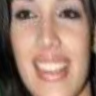
\includegraphics[scale = 0.2]{../../proposal/face_photos/Amelia_Vega_0001.png} &  
  $\vec{z}_2^{(1)} = $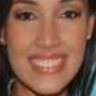
\includegraphics[scale = 0.2]{../../proposal/face_photos/Amelia_Vega_0002.png} &  
  $\vec{z}_3^{(1)} = $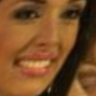
\includegraphics[scale = 0.2]{../../proposal/face_photos/Amelia_Vega_0003.png} &  
  $\vec{z}_*^{(1)} = $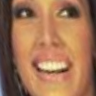
\includegraphics[scale = 0.2]{../../proposal/face_photos/Amelia_Vega_0004.png} \\ \hline
$y^{(2)}$=Jean-Pierre & 
  $\vec{z}_1^{(2)} = $
\includegraphics[scale = 0.2]{../../proposal/face_photos/Jean-Pierre_Raffarin_0001.png} &  
  $\vec{z}_2^{(2)} = $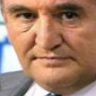
\includegraphics[scale = 0.2]{../../proposal/face_photos/Jean-Pierre_Raffarin_0002.png} &  
  $\vec{z}_3^{(2)} = $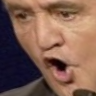
\includegraphics[scale = 0.2]{../../proposal/face_photos/Jean-Pierre_Raffarin_0003.png} &  
  $\vec{z}_*^{(2)} = $
\includegraphics[scale = 0.2]{../../proposal/face_photos/Jean-Pierre_Raffarin_0004.png} \\ \hline
$y^{(3)}$=Liza & 
  $\vec{z}_1^{(3)} = $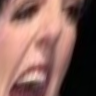
\includegraphics[scale = 0.2]{../../proposal/face_photos/Liza_Minnelli_0001.png} &  
  $\vec{z}_2^{(3)} = $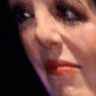
\includegraphics[scale = 0.2]{../../proposal/face_photos/Liza_Minnelli_0002.png} &  
  $\vec{z}_3^{(3)} = $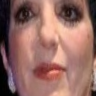
\includegraphics[scale = 0.2]{../../proposal/face_photos/Liza_Minnelli_0003.png} &  
  $\vec{z}_4^{(3)} = $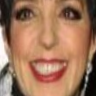
\includegraphics[scale = 0.2]{../../proposal/face_photos/Liza_Minnelli_0004.png} \\ \hline
$y^{(4)}$=Patricia & 
  $\vec{z}_1^{(4)} = $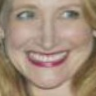
\includegraphics[scale = 0.2]{../../proposal/face_photos/Patricia_Clarkson_0001.png} &  
  $\vec{z}_2^{(4)} = $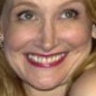
\includegraphics[scale = 0.2]{../../proposal/face_photos/Patricia_Clarkson_0002.png} &  
  $\vec{z}_3^{(4)} = $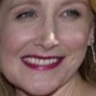
\includegraphics[scale = 0.2]{../../proposal/face_photos/Patricia_Clarkson_0003.png} &  
  $\vec{z}_4^{(4)} = $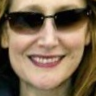
\includegraphics[scale = 0.2]{../../proposal/face_photos/Patricia_Clarkson_0004.png} \\ \hline
\end{tabular}
\caption{Face recognition problem}
\label{fig:face_rec}
\end{figure}

Decades of research into facial recognition has confirmed that careful
\emph{feature-engineering} or \emph{representation-learning} is the
key to acheiving human-level performance on the face recognition task.
The feature-engineering approach involves crafting algorithms to
locate landmarks in the image (the corners of the eyes, nose, mouth,
etc.) and to use distances between landmarks as features.  The most
sophisticated approaches extract features by means of first fitting a
three-dimensional model of the face to the photograph.

More recently, fully automated feature-learning, or
\emph{representation-learning}, using deep convolutional networks
(CNN) has yielded record performance.  Google's FaceNet
(\cite{schroff2015facenet}), using learned features from a deep CNN,
acheived an accuracy of $0.9964 \pm 0.0009$ on the Labeled Faces in
the Wild (LFW) benchmark dataset, outperforming Facebook's DeepFace
(which uses both a deep CNN, and 3D modeling, with an accuracy of
$0.9735 \pm 0.0025$, \cite{taigman2014deepface}) and a human benchmark
(accuracy 0.9753, \cite{kumar2009attribute}).

\begin{figure}
\centering
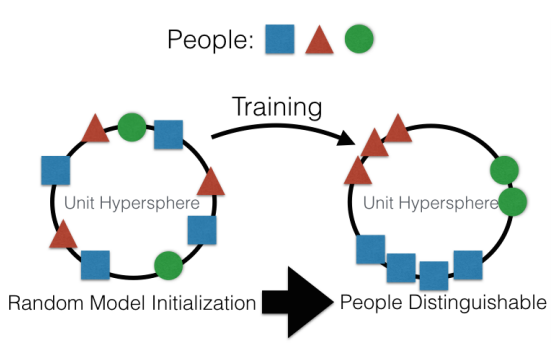
\includegraphics[scale = 0.5]{Figures/triplet_loss.png}
\caption{Triplet loss function for training face representations.  From \cite{amos2016openface}}
\label{fig:triplet_loss}
\end{figure}

The method that FaceNet uses to learn a representation
$\vec{g}(\vec{z})$ (a collection of nonlinear mappings of the input
image) is highly interesting.  The representation $\vec{g}$ is
parameterized by a deep CNN architecture: in other words, the basis
functions $g_i$ are the end result of composing several layers of
nonlinear transformations as specified by the hierarichical
architecture of the CNN.  However, for our purposes, the modeling and
algorithmic details of the CNN are not important, and we refer the
interested reader to [CITE] for a reference on principles of
convolutional neural networks.  At a higher level of abstraction, we
can say that the representation $\vec{g}_\theta(\vec{z})$ lies in a
class of nonlinear functions, parameterized by some (possibly large)
vector of parameters, $\theta$.  The triplet loss function used by
FaceNet defines the objective function used to estimate $\theta$ and
therefore find a good representation.

The intuition behind the triplet loss function is that a good
representation $\vec{g}(\vec{z})$ should cause faces of the same
person to cluster, as illustrated in Figure \ref{fig:triplet_loss}.
Therefore, the triplet loss function encourages inputs $\vec{z},
\vec{z}'$ that belong to the same class (that is, faces which belong
to the same person) to have a representations $\vec{g}(\vec{z}),
\vec{g}(\vec{z}')$ that are close to each other in terms of Euclidean
distance, while inputs $\vec{z}, \vec{z}^*$ which belong to different
classes are encouraged to have representations $\vec{g}(\vec{z}),
\vec{g}(\vec{z}^*)$ which are far apart in terms of Euclidean
distance.  Note also that for the triplet loss, we require the
representations $\vec{g}$ to be normalized to have unit norm, so that
the maximum distance between two representations is 2.

Recall that the training data consists of images $\{\vec{z}_j^{(i)}\}$
where $i$ indexes the person (or class) and $j$ indexes the repeats
from the same class.  Define a \emph{triplet} as a triple consisting
of an \emph{anchor}, a \emph{positive example} from the same class as
the anchor, and a \emph{negative example} from a different class from
the anchor,
\[
(\underbrace{\vec{z}_j^{(i)}}_{\text{anchor}}, \underbrace{\vec{z}_k^{(i)}}_{\text{positive example}}, \underbrace{\vec{z}_\ell^{(m)}}_{\text{negative example}})
\]
where $j \neq k$ and $m \neq i$.  For instance, in a training set with
$N$ classes and $M$ training examples per class, we can form
$N(N-1)M^2(M-1)$ triplets.  The triplet loss is then defined as
\[
\text{TripletLoss}_{\theta} = \sum_{j \neq k} \sum_{m \neq i} \sum_\ell 
[||\vec{g}_\theta(\vec{z}_j^{(i)}) - \vec{g}_\theta(\vec{z}_k^{(i)})||^2 + \alpha
 - ||\vec{g}_\theta(\vec{z}_j^{(i)}) - \vec{g}_\theta(\vec{z}_\ell^{(m)})||^2]_+
\]
where $\alpha$ is a tuning parameter (defining the desired separation
between inter-cluster distance and between-cluster distance).  In the
case of FaceNet, stochastic gradient descent with backpropagation is
used to update the CNN parameters $\theta$ over mini-batches of
triplets.

\subsection{What makes a good representation?}

One of the big questions in representation learning is how to define
or evaluate the quality of a
representation\cite{bengio2013representation}.  When, as in face
recognition, the end goal of the representation learning is to obtain
more accurate predictions or classifications within a machine learning
pipeline, an obvious criterion for the quality of the representation
is the prediction or classification accuracy that can be attained
after using that particular representation as the feature set for a
classification or regression model.

However, this result-oriented approach to evaluating representations
has two drawbacks.  Firstly, it may be difficult to work with a
performance metric (such classification or regression accuracy) as a
quality metric, since obtaining the performance metric requires
training a model and then testing it on data, which can be
computationally costly and may not yield a differentiable objective
function.  Secondly, one of the appealing qualities of a `good'
representation is that it should enable good performance in a
\emph{variety} of different tasks.  Limiting the definition of `good'
to performance on a single task seemingly ignores the requirement that
a representation should be general across tasks.

%% sufficient statistics in parametric stats?

Thinking about generative models suggests different avenues for
evaluating representations.  One such generative model is that the
observations $\vec{z}$ (e.g. images of faces) originate from some
latent objects $\vec{t}$ (e.g. a person's head).  We can think of the
observations $\vec{z}$ as being generated by some mechanism which
depends on the attributes of the latent objects, $\vec{t}$, as well as
some \emph{nuisance parameters} or \emph{degrees of freedom}
$\vec{\xi}$ (such as the pose, or lighting of the face) which modulate
how the features of $\vec{t}$ are expressed (or perhaps masked) in the
observed data $\vec{z}$.  Presumably, for the task at hand,
e.g. identifying the person, only the latent objects $\vec{t}$ are
important, and not the nuisance parameters.  However, it is worth
noting that for a different task, such as `pose identification'
(rather than face identification) it may be the case that the roles of
the nusiance parameters $\vec{\xi}$ and the latent objects $\vec{t}$
are switched--as the saying goes, one man's signal is another man's
noise.

\cite{bengio2013representation} suggest that an ideal representation,
rather than discriminating between `signal' and `noise', would serve
to \emph{disentangle} the effects of \emph{all factors} without
throwing away any information.  In other words, an ideal
representation would map $\vec{z}$ onto some estimate of $(\vec{t},
\vec{\xi})$ which separates the effect of the latent objects from
nuisance parameters, and also allows for \emph{reconstruction} of
observation from the representation.  We will come across similar
ideas when we discuss \emph{auto-encoders} in the related work
section.

However, in this work, we take a more simplistic approach, where we
\emph{enforce} a distinction between one set of factors, $\vec{t}$, as
the `signal', and $\vec{\xi}$ as the `noise', and where we are happy
with a representation that keeps the signal while discarding the
noise. The `signal-only' approach to representations is sufficient for
most current applications, including the two examples of
`representation evaluation' that we just presented--the facial
recognition problem, and the evaluation of receptive field models in
fMRI data.

In the case of facial recognition, the `signal' is the features of the
face that persist across different perspectives and illumination,
while the `noise' is the effect of pose, illumination, transient
features such as hairstyle and makeup, and occlusive accesories such
as sunglasses.  
%One might imagine that an idealized representation for
%facial recognition is one that estimates the latent, persistent
%traits, such as the shape and size of facial features, while
%discarding the effects of `nuisance' parameters such as pose and
%lighting.  
The effect of extracting the signal while reducing the
noise is to shrink inputs that share the same latent variables--faces
from the same person--towards each other, as illustrated in Figure
\ref{fig:triplet_loss}.

Meanwhile, in the case of the functional MRI study, it is the V1
neurons themselves which define what is the `signal' and what is the
`noise' in the input.  The V1 neurons only respond to certain features
in the data, and ignore others.  Therefore, the goal of the receptive
field model is to extract the information in the data that is relevant
to V1 (such as, perhaps, local angular frequencies in the image) and
discard other information (e.g. intensities of individual pixels).

In both examples, we have not have inputs $\vec{z}$ but also some form
of \emph{side information} that helps us distinguish between signal
and noise.  In the case of facial recognition, the side information is
the labels $y$ which label the photographs.  In the case of the
functional MRI study, the side information is the V1 intensities
$\vec{y}^{V1}$ which give us information as to what V1 neurons ``care
about'' in the image.

The unifying theme of this thesis is how to evaluate (possibly
nonlinear) representations $\vec{g}(\vec{z})$ of inputs $\vec{z}$ when
we are given pairs $(\vec{z}_i, y_i)$ of input vectors as well as some
form of `side-information' $y_i$, which we will call \emph{the
  response variable}, that gives us some basis for distinguishing
signal from noise.  As we will explain further in the ensuring
chapters, we consider three different methods for evaluating the
quality of the representation.

\begin{enumerate}
\item The \emph{mutual information} $I(\vec{g}(\vec{Z}); Y)$ between the representation
and the response variable.
\item In the case of discrete response variables $Y$: 
the $k$-class average classification accuracy.
\item In the case of continuous response variables $Y$:
the \emph{identification accuracy.}
\end{enumerate}

The mutual information is a classical measure of dependence that was
first developed by Claude Shannon as one of the key concepts in
information theory.  The $k$-class average classification accuracy is
a concept that has not been (to our knowledge) previously introduced
in the literature, but it is highly related to the
\emph{identification accuracy}, which was introduced by the same
functional MRI study of natural images (\cite{Kay2008a}) that we have
been discussing.  To our knowledge, we are the first to investigate
the properties of the identification task from a theoretical
perspective.

All three of these methods enable \emph{supervised evaluation of
  representations} because they define a quality metric which depends
on a response variable $Y$.  As in \emph{supervised learning}, the
response $Y$ gives us a means of judging the quality of the
representation $\vec{g}(\vec{z})$.

Comparing these methods, the advantage of the $k$-class average
classification accuracy or identification accuracy is that they are
relatively easy to compute, even in high-dimensional data, because one
can make use of machine-learning methods for computing these
quantities.  Meanwhile, the mutual information is extremely difficult
to estimate in high-dimensional data.  However, the advantage of the
mutual information is that it does not depend on arbitrary tuning
parameters, while both the $k$-class average classification accuracy
and identification risk depend on the choice of a tuning parameter
$k$.

However, one of the main theoretical contributions of this work is to
show how all of these three methods: mutual information, $k$-class
average classification accuracy, and identification accuracy, are
highly related.  In particular, we establish methods for
lower-bounding the mutual information from either the $k$-class
average classification accuracy or identification accuracy.

\subsection{Related Work}

As we hoped to convey in the introduction, the problem of finding and
evaluating representations is an extremely hot topic in multiple
disciplines, from neuroscience to machine learning.  Consequently, the
space of possible approaches to the problem is vast.  We limit our
study to a few highly interconnected and (in our opinion) interesting
approaches to the problem of evaluating representations, in the
special case when a \emph{response} variable $Y$ is available and
where one wants to take advantage of the side-information provided by
this response.

However, many other ideas exist for evaluating representations.  One
extremely notable family of approaches, which lies totally outside the
scope of this thesis, is \emph{unsupervised} methods for evaluating
representations-- methods which do not require access to an external
response variable $Y$.  Obviously, this is highly interesting, because
in many applications one does not have easy access to such a response
variable.  One family of methods--including restricted Boltzmann
machines and gaussian restricted Boltzmann machines--fits a parametric
distribution to the inputs $\vec{z}$ [CITE].  The representations are
obtained as summary statistics of the latent variables in the model,
and the quality of the representation is assessed via tha
\emph{likelihood} of the parametric model.  \emph{Auto-encoders} form
another family of methods [CITE].  Representations, or \emph{encoders}
$\vec{g}$ are paired with \emph{decoders} $\vec{g}^{-1}$ that infer
the original input from the representation.  The quality of the
representation $\vec{g}$ is based on the reconstruction error obtained
by comparing the original input to the inverse of the representation,
\[
||\vec{z} - \vec{g}^{-1}(\vec{g}(\vec{z}))||^2.
\]
In the case that $\vec{g}$ is of smaller dimensionality than
$\vec{z}$, this forces the representation to extract highly
explanatory `latent factors' that explain most of the variation in
$\vec{z}$.  (If this sounds familiar, it may be because Principal
Component Analysis can be interpreted as an auto-encoder model: the
principal components minimize the reconstruction error over all linear
encoding/decoding rules.)  However, one can also consider
\emph{over-complete} representations of higher dimensionality than
$\vec{z}$.  In order to prevent the identity map (which would
trivially have zero reconstruction error) from being the optimal
representation, a variety of different approaches can be taken to
modify the objective function.  One is to require the auto-encoder
(the composition of the encoder and decoder) to recover the original
input $\vec{z}$ from a \emph{noisy} input $\tilde{z} = \vec{z} +
\vec{\epsilon}$.  Another approach is to \emph{regularize} the
encoder, for instance, requiring sparsity in the output of the
encoder.

With regards to \emph{supervised} evaluation of representations, one
can find extremely similar ideas in the methodology of
\emph{representation-similarity analysis}, which was introduced by
\cite{kriegeskorte2008representational} to the neuroscience community,
and which has already grown incredibly popular within the field given
the short span of time since its introduction.  However, the
methodology is based on much more classical work in statistics and
psychometrics on \emph{distance-based inference}.  The idea is that if
one has multiple \emph{views} of the same object, say, the pixel
values $\vec{z}_i$ of an image, a semantic labeling $y_i$ (`house' or
`chair'), as well as a subject's response $\vec{x}_i$ to the image, as
measured by fMRI, then all of these different views can be
\emph{compared} by means of their \emph{inter-object distance
  matrices.}  That is, if we have distinct objects indexed by $i =
1,\hdots, n$, then one can form an $n \times n$ distance matrix for
each view: for instance, $D_{\vec{z}}$, the matrix of all pairwise
Euclidean distances between pixel vectors; $D_{y}$, a binary matrix
indicating pairs of identical labels with 0 and non-identical labels
with 1; and $D_{\vec{x}}$, a matrix of pariwise Euclidean distances
between fMRI images.  One can then compare these resulting distance
matrices (e.g. in terms of correlation) to determine which
\emph{views} are similar to each other, and which are dissimilar.  For
instance, one may find that distances within `brain-space',
$D_{\vec{x}}$, are much more similar to semantic distances $D_{y}$
than raw pixel distances $D_{\vec{z}}$.

One could easily adapt the ideas in representational-similarity
analysis towards the supervised evaluation of representations.  A
representation $\vec{g}$ is good if the resulting distance matrix
$D_{\vec{g}}$ of pairwise distances between representations is similar
to the distance matrix $D_y$ between responses.  In fact, one could
interpret the \emph{triplet-loss} objective function as enforcing a
kind of \emph{representational similarity} between face
representations $\vec{g}(\vec{z})$ and labels $y$.  Two faces with the
same label have a distance of 0 within $D_y$, and therefore, they
should have a small distance within $D_{\vec{g}}$.  Two faces with
different labels have distance 1 within $D_y$; therefore, they should
have at least $\alpha$ distance within $D_{\vec{g}}$.

However, the connection between representational-similarity analysis
and supervised evaluation of representations remains unexplored in
this work.  We leave it to future research.

\section{Overview}

\subsection{Theme and variations}

We have seen that the main \emph{theme} of the thesis is the
supervised evaluation of representations.  However, a number
of \emph{subthemes} arise from similar problems in related
disciplines, and additional applications of our methods.

\emph{Subtheme: Recognition systems}.  We have seen that
\emph{recognition systems}, such as facial recognition systems, which
are tasked with identifying objects from data, depend on finding a
good representation of the data.  Recognition systems and
representations are also highly linked because one way to define `what
makes a good representation?' is that a good representation should
enable accurate recognition.  However, one issue that a formal
definition of how to evaluate the quality of a recognition system has
been missing in the literature.  Our proposals for modelling
recognition problems, and for evaluating recognition systems, is
through the formalism of \emph{randomized classification}, which
defines parameters for multi-class classification problems (think of
the problem of classifying a face to $K$ possible people) where the
classes have been drawn randomly.

\emph{Subtheme: Information geometry}.  An intuitive notion of quality
for representations is that the distance between representations
should reflect \emph{meaningful differences} (or `signal') between the
underlying objects $\vec{t}$ rather than the effect of the degrees of
freedom $\vec{\xi}$ in the representation.  However, the proper
measure of distance in the representation space is arguably the
\emph{statistical distance} rather than geometric (e.g. Euclidean)
distance.  That is, if we consider the nuisance parameters $\vec{\xi}$
as random variables, then the distance between a representations
$\vec{g}(\vec{z})$ and $\vec{g}(\vec{z}')$ should reflect the power
with which we can conduct a \emph{statistical hypothesis test} for
determining whether the representations originate from the same latent objects, 
\[
H_0: \vec{t} = \vec{t}'.
\]
The leads us to consider the ideas in \emph{information geometry},
which is the study of spaces of \emph{distributions}
$\{f_\theta\}_{\theta \in \Theta}$ in which distance is measured by
some type of statistical distance or divergence, e.g. Kullback-Liebler
divergence (\cite{amari2007methods}).  To fit our problem into the
framework of information geometry, we would consider the latent
objects $\vec{t}$ as playing the role of the parameter $\theta$, and
the induced distribution of $\vec{g}(\vec{z})$ as the distribution
$f_\theta$.  It is important to note however, that this the emphasis
on parameter spaces is complemented by the concept of \emph{duality}
between the space of distributions and the space of observations.  The
concept can be formalized in exponential families, where a sample from
$f_\theta$ can be represented in the distributional space as the MLE
estimate $f_{\hat{\theta}}$, and where the process of estimation is
seen to correspond to projection operators.

Within this framework, one can consider the \emph{metric
  entropy} of a space $\Theta$, which is a measure of the
\emph{volume} of the space according to statistical distance.  A ball
$B_{\theta, r}$ centered at parameter $\theta$ and with radius $r$ is
defined as the set of parameters $\theta'$ such that the statistical
distance between $f_\theta$ and $f_{\theta'}$ is less than $r$:
\[d(f_{\theta}, f_{\theta}) < r.\]
The $\delta$-\emph{metric entropy} of the space $\Theta$ is defined as
the minimum number of balls of radius $\delta$ needed to cover
$\Theta$ (\cite{adler2009random}).  While we will not employ the
formal tools of information theory in this work, we take inspiration
from some of the intuitions.  Instead, we use \emph{information
  theory}, a closely related field, to provide much of the formalism
for our theory.

\emph{Subtheme: Information theory}.  Extremely similar notions of
\emph{volume} appear in information theory, which is the study of how
to design systems for transmitting messages between a sender and a
reciever over a possibly noisy channel.  We will review more of the
background of information theory later in this chapter.  For now, we
note that the analogy between information theory and information
geometry is that now the \emph{encoded message} plays the role of the
parameter $\theta$, and we are concerned with the space of the
distributions $f_\theta$ of \emph{recieved messages}.  The
\emph{capacity} of a channel is a measure of the \emph{volume} of the
space.  The channel capacity is defined in terms of \emph{mutual
  information}, which plays the analogue of the logarithm of the
\emph{metric entropy}.  This can be seen clearly if we consider the
Euclidean case for metric entropy: the log-metric entropy is closely
related to the difference of the log-volume of the space and the
log-volume of the ball $B_{\theta, \delta}$.  Meanwhile, mutual
information $I(T; R)$ is defined as the difference between the entropy of $R$ (the recived message)
and the conditional entropy of $R$ given $T$ (the transmitted message):
\[
I(T; R) \stackrel{def}{=} \underbrace{H(R)}_{\text{entropy}} - \underbrace{H(R|T)}_{\text{conditional entropy}}.
\]
Here the entropy $H(R)$ is analagous to the log-volume of the entire
space, while the conditional entropy $H(R|T)$ measures to log-volume
of the ball which is centered at the parameter $T$.  While mutual
information is not defined explicitly in terms of packing or covering
numbers, as we see in the Euclidean example for metric entropy, both
packing and covering numbers are approximately equivalent to volume
ratios.  Another difference between the mutual information and the
metric entropy is that the mutual information is concerned with volume
in the \emph{observation} space (the space of recieved messages $R$)
rather than the \emph{parameter space}.  However, due to the concept
of duality, we can see that one arrives at similar definitions of
volume whether we choose to use the parameter space, or its dual, the
observation space.

\emph{Subtheme: Estimation of mutual information.}  Besides serving
(in our case) as a measure of statistical volume, the mutual
information enjoys numerous other desirable properties such as
symmetry, invariance under bijections, and independent additivity, as
we will review later in the chapter.  Due to these properties, the
mutual information is an ideal measure of dependence for many
problems; therefore, in a variety of applications, including many in
neuroscience, it is desirable to estimate the mutual information of
some empirically observed joint distribution.  However, this is a
highly nontrivial functional estimation problem in high dimensions.
By connecting mutual information to more easily estimated quantities
such as average classification accuracy, our work provides novel
estimators of mutual information, which we show to have better scaling
properties in many high-dimensional problems than previous approaches
for estimating mutual information.

\emph{Subtheme: Connections between information theory and supervised
  learning}.  Information theory, statistics, and machine learning
have many interconnections, as testified by the many applications of
information-theoretic inqualities in statistical and machine learning
research.  By studying both information-theoretic and
classification-based methods for evaluating representations, we
uncover additional links between information theory and
classification.  Fano's inequality, which bounds the mutual
information in terms of Bayes accuracy of classification
($\text{BA}$),
\[
\text{I}(X; Y) \geq = \log(k)-H(\text{BA}) - (1-\text{BA})\log(k-1),
\] 
is one of the earliest results bridging the two worlds of information
theory and supervised learning.  However, its application is limited
to \emph{discrete} and \emph{uniformly} distributed $X$.  Our work in
Chapter 4 provides an extension of Fano's inequality to the case of
continuous $(X, Y)$, through means of the Bayes accuracy of
\emph{identification}.

\emph{Subtheme: Geometric inference from random samples.}  Regardless
of which definition of `volume' one employs, a natural question is how
to estimate this `volume' from empirical data.  That is, we wish to
infer a geometric characteristic of the space--the volume--from a
random sample of observations drawn from the space.  Meanwhile, a
complementary question that was already extensively studied in
information theory is the question of how to \emph{construct} a
collection of points in the random space that \emph{optimizes} another
geometric characteristic--the overlap between points.  It was
established by Shannon that the \emph{randomization} method provides
such a construction--a randomly drawn collection of points has
asymptotically optimal properties in terms of maximum overlap (as
measured by decoding error.)  In information theory, these random
constructions pioneered by Shannon continued to be studied in the form
of \emph{random code models}.

Returning to the problem of inferring volume from samples, two
questions arise--one being how to construct an estimator, and
secondly, what is the variance of the estimator.  We define volume in
terms of mutual information and develop estimators based on
\emph{random classification tasks}, which specify the sampling
mechanism.  Furthermore, we obtain preliminary results on the
variability of such estimators.  We compare our results to existing
results in information theory regarding random code models.

\emph{Subtheme: Generalizability of experiments.} Two of our
motivations for studying random classification tasks is (i) to
evaluate representations, and (ii) as a model for recognition
problems.  Yet a third application is for understanding the
generalizability of experiments that can be modelled as random
classification tasks.  For example, many task-fMRI experiments can be
modelled random classification tasks, because the stimuli sets used in
the experiment are composed of arbitrary (`random') exemplars, and
therefore the stimuli set used by one lab may differ from the stimuli
set used by another lab, even when they are presumably studying the
same task.  Intuitively, using larger and more diverse stimuli sets
should lead to better generalizability of results to the entire
population of stimuli.  Our work on random classification--in
particular, our variance bounds on the classification accuracy in
randomized classification tasks--provides a theoretical basis for
understanding how well the results of a random classification task
allows inference to population parameters, such as the mutual
information between the stimulus and the response.

\subsection{Organization}

The rest of the thesis is organized as follows.  The remaining
sections in this chapter deal with background material on supervised
learning and information theory, as well as the application of both to
neuroscience, which forms a major motivation for the current work.
Chapter 2 introduces the concept of randomized classification, and
also establishes some variability bounds which will be used later in
the development of inference procedures.  Chapter 3 studies the
dependence of classification accuracy on the label set size in
randomized classification, and a practical method for predicting the
accuracy-versus-label set size curve from real data.  Chapter 4 and 5
deal with the applications of randomized classification to the
estimation of mutual information in continuous data: chapter 4 derives
a lower confidence bound for mutual information under very weak
assumptions, while chapter 5 works within an asymptotic
high-dimensional framework which leads to a more powerful but less
robust estimator estimate of mutual information.


\subsection{Note on attribution}

The content in chapters 1,2, 4, and 5 is based on joint work with
Yuval Benjamini.  Chapter 3 is based on joint work with Yuval
Benjamini and Rakesh Achanta.  All theoretical results are due to the
author.

\section{Information and Discrimination}

%\subsection{Overview}

We now begin our review of background material in supervised learning
and information theory.  Therefore, a reader who is familiar to both
fields could skip most of the following--with the exception of the
explanation of \emph{identification accuracy} in section
\ref{sec:ident_risk}, which is a relatively novel concept in
the statistical literature.  Also, we hope that even the experienced
reader will find some food for thought in our comparison of
information theory and supervised learning, and our humble
speculations about how current developments may increase the degree of
interaction between the two areas.

\subsection{Introduction}

In studying the problem of evaluating representations, we make use of
two closely related frameworks: firstly, the multi-class
classification framework from the statistics and machine learning
literature, and secondly, the concepts of information theory.  From a
broader perspective, this is hardly unusual, since concepts such as
entropy, divergence, and mutual information are commonly applied in
theoretical statistics and machine learning.  Furthermore, information
theory, theoretical statistics, and machine learning are based on the
same foundation: measure-theoretic probability theory; one could even
say that all three disciplines are subfields of applied probability.
However, while the three sub-fields may appear very similar from a
mathematical perspective, some differences arise if we examine the
kinds of intuitions and assumptions that are characteristic of the
literature in each area.

A common problem to all three subfields is the inference of some
unobserved quantity on the basis of observed quantities.  In classical
statistics, the problem is to infer an unknown parameter; in
supervised learning, the problem is to predict an unobserved label or
response $Y$; in information theory, the problem is to decode a noisy
message.  Next, the metric for quantifying achievable performance
differs between the three disciplines.  In classical statistics, one
is concerned with the variance of the estimated parameter, or
equivalently, the Fisher information.  In machine learning, one seeks
to minimize (in expectation) a \emph{loss} function which measures the
discrepancy between the prediction and the truth.  In information
theory, one can measure the quality of the noisy channel (and
therefore, the resulting achievable accuracy) through the \emph{mutual
  information} $I(X; Y)$ between the sender's encoded message $X$ and
the reciever's recieved message $Y$.  If we specialize within machine
learning to the study of classification, then we are concerned with
accurate \emph{discrimination} of the input $X$ according to labels
$Y$.  Similarly, if we specialize to the problem of hypothesis testing
within statistics, the the problem is again to \emph{discriminate}
between two (or more) different hypotheses regarding the
data-geenrating mechanism.

%% have to reorder the next para, 
The concepts of \emph{information} and \emph{discrimination} are quite
distinct from an intuitive standpoint; however, they are linked at a
fundamental level.  This link can be seen throughout statistics and
machine learning, and in the way we think about statistical problems.
A statistical hypothesis test is \emph{informative} because it
provides evidence that the data behaves according to a certain
hypothesis rather than another.  %% slightly redundant with prev para.
In information theory, even if the reciever cannot conclusively
determine the sender's message from the observed signal, the signal
still contains \emph{information} if it contains some evidence that
favors one set of possible messages over another.  The formalism of
measure-theoretic probability theory provides yet another example of
the conceptual link between information and
discrimination\footnote{Supposing $\Omega$ is a probability space
  defined with respect to a $\sigma$-algebra $\mathcal{F}$, we can
  represent our state of knowledge with a filtration (or
  sub-$\sigma$-algebra) $\mathcal{F}' \subseteq \mathcal{F}$.
  Complete knowledge (zero uncertainty) is represented by the full
  $\sigma$-algebra: that is, $\mathcal{F}' = \mathcal{F}$.  Partial
  knowledge is represented by a coarser filtration, $\mathcal{F}
  \subset \mathcal{F}'$.  The filtration, of course, indicates that
  our knowledge is sufficient to \emph{discriminate} the outcome space
  $\Omega$ into a number of finitely or infinitely many categories.
  The more information we have, (or, the closer we come to complete
  knowledge of the outcome), the more finely we can discriminate the
  realized outcomes given by $\omega \in \Omega$.}.

%% the purpose of this paragraph is to make the link between discrimination and information
%% this para needs work after being moved
Either natural or artificially intelligence recognition systems must
rely on input data that is \emph{informative} of the optimal response
if they are to achieve reasonable discriminative accuracy.  In natural
environments, mammals rely on a combination of visual, auditory, and
tactile cues to recognize potential threats in the environment.
Mammalian brains integrate all of this sensory information in order to
make more rapid and reliable decisions.  Generally, increased
diversity and quality of the available sources of information will
lead to more accurate recognition (say, of possible environmental
threats.)

This link between the information content of the input and the
achievable discrimination accuracy was first quantified by Claude
Shannon via the concept of \emph{mutual information.}  The mutual
information $I(X; Y)$ quantifies the information content that an input
$X$ holds abut a target of interest, $Y$.  For instance, in the case
of facial identification, the discrimination target $Y$ is a label
corresponding to the identity of the person, and $X$ is an image of
the individual's face.  An image corrupted by noise holds less
information, and correspondingly leads to lower classification
accuracies.

The discrmination problem that Shannon studied--the
\emph{noisy-channel decoding problem}, is extremely similar to the
multi-class classification problem, but also features some important
differences.  A side-by side comparison between the schematics of
multi-class classification and the noisy channel problem is displayed
in Figure \ref{fig:mcc_vs_it}.  We will elaborate much further on the
comparison illustrated in the figure, but for now, one can note that
both the multi-class classification problem and the noisy-channel
decoding problem involves the inference of a latent variable $Y$ from
an observation $X$, where $X$ is linked to $Y$ through a conditional
distribution $F_Y$.

\tikzstyle{block} = [rectangle, draw, fill=white, 
    text width=5em, text centered, rounded corners, minimum height=4em]
\tikzstyle{cloud} = [ellipse, draw, fill=white, 
    text width=5em, text centered, rounded corners, minimum height=4em]
\tikzstyle{line} = [draw, -latex']
    
\begin{figure}
\centering
\begin{tabular}{ccc}

Multi-class classification & & Information Theory\\

\begin{tikzpicture}[node distance = 2cm, auto]
    % Place nodes
    \node [block] (init1) {label $Y$};
    \node [cloud, below of=init1] (init2) {distribution $F_Y$};
    \node [block, below of=init2] (init3) {observation $X$};
    \node [cloud, below of=init3] (init4) {classification rule $h(X)$};
    \node [block, below of=init4] (init5) {estimate $\hat{Y}$};
    % Draw edges
    \path [line] (init1) -- (init2);
    \path [line] (init2) -- (init3);
    \path [line] (init3) -- (init4);
    \path [line] (init4) -- (init5);
\end{tikzpicture} 

& & 

\begin{tikzpicture}[node distance = 2cm, auto]
    % Place nodes
    \node [block] (initA) {message $M$};
    \node [cloud, below of=initA] (initB) {encoder $g(M)$};
    \node [block, below of=initB] (init1) {encoded message $Y$};
    \node [cloud, below of=init1] (init2) {noisy channel $F_Y$};
    \node [block, below of=init2] (init3) {observation $X$};
    \node [cloud, below of=init3] (init4) {decoder $d(X)$};
    \node [block, below of=init4] (init5) {estimate $\hat{M}$};
    % Draw edges
    \path [line] (initA) -- (initB);
    \path [line] (initB) -- (init1);
    \path [line] (init1) -- (init2);
    \path [line] (init2) -- (init3);
    \path [line] (init3) -- (init4);
    \path [line] (init4) -- (init5);
\end{tikzpicture} 

\end{tabular}
\caption{Comparing the discrimination tasks in multi-class classification and information theory.}
\label{fig:mcc_vs_it}
\end{figure}

We will now briefly review the relevant background for supervised learning and
information theory, to give the context for each side of figure
\ref{fig:mcc_vs_it}.  Afterwards, we will compare and contrast the
supervised learning and information theory, and note what kind of
cross-talk exists between the two related fields, and what new
developments could still arise by way of a dialogue between supervised
learning and information theory.  One such new development is the
\emph{randomized classification} model, since it is a very close
analogue of the \emph{random code} model studied in information
theory.

\subsection{Supervised learning}

Up until now we have been discussing \emph{classification}, which is a
particular type of \emph{prediction task}.  However, the most general
recipe for a prediction task involves:

\begin{itemize}
\item A predictor space $\mathcal{X}$ defining the possible values the
  predictor $X$ can take; though typically, $\mathcal{X} =
  \mathbb{R}^p$.
\item A response space $\mathcal{Y}$ defining the possible values the response $Y$ can take;
\item An \emph{unknown} population joint distribution $G$ for the pair $(\vec{X}, Y)$;
\item A \emph{cost} function defining the penalty for incorrect
  predictions, $C: \mathcal{Y} \times \mathcal{Y} \to \mathbb{R}$.  If
  $Y$ is the response, and $\hat{Y} = h(\vec{X})$ is the prediction, then
  the loss for making the prediction $\hat{Y}$ when the truth is $Y$
  is given by $C(Y; \hat{Y})$.
\end{itemize}

The various types of prediction tasks include classification,
regression, and multivariate variants: such as multi-label
classification and multiple-response regression.  These special cases
are just specializations of the general prediction task to a
particular type of response space.

\begin{itemize}
\item In \emph{classification}, the response space is finite and
  discrete.  In \emph{binary classification}, the response space
  $\mathcal{Y}$ consists of two elements, say, $\mathcal{Y} = \{0,
  1\}$.  Multi-class classification usually refers to the case
  $\mathcal{Y}$ has more than two elements.  The most common cost
  function for classification is zero-one loss,
\[
C(y; \hat{y}) = I(y \neq \hat{y}).
\]
\item In \emph{regression}, the response space is $\mathbb{R}$.  The most common cost function is squared loss:
\[
C(y; \hat{y}) = (y - \hat{y})^2.
\]
\item In \emph{multi-label classification}, the response space is a
  product of several finite sets, say $\mathcal{Y} = \mathcal{Y}_1
  \times \mathcal{Y}_2 \times \cdots \mathcal{Y}_\ell$.  That is to
  say, that the response $\vec{Y}$ consists of a categorical vector,
  $\vec{Y} = (Y_1,\hdots, Y_\ell)$. More complex types of cost
  functions can be considered, such as \emph{Jaccard distance},
\[
C(\vec{y}; \hat{\vec{y}}) = \frac{\sum_{i=1}^\ell y_i \wedge \hat{y}_i}{\sum_{i=1}^\ell y_i \vee \hat{y}_i}.
\]
\item In \emph{multiple-response regression}, the response space is $\mathbb{R}^p$.  A natural cost function is squared Euclidean distance,
\[
C(\vec{y}; \hat{\vec{y}}) = ||\vec{y} - \hat{\vec{y}}||^2.
\]
\end{itemize}

A \emph{prediction rule} is a function $h: \mathcal{X} \to
\mathcal{Y}$ for predicting $Y$ as a function of $\vec{X}$.
Prediction rules can be found through a variety of means.  In some
domains, experts manually construct the prediction rules using their
domain knowledge.  However, the field of \emph{supervised learning}
aims to algorithmically construct, or `learn' a good prediction rule
from data.  In supervised learning, we assume that we have access to a
\emph{training set} consisting of $n_1$ observations
$\{(\vec{X}_i,Y_i)\}_{i=1}^{n_1}$, plus a \emph{test set} consisting
of $n_2$ observations $\{(\vec{X}_i,Y_i\}_{i=n_1 + 1}^{n_1 + n_2}$;
usually, we assume that the pairs in both the training and test set
have been sampled i.i.d. from the distribution $G$.  As we will
elaborate further, the training set is used to construct $h$, while
the test set is used to evaluate the performance of $h$.
%We will also write $\bX$
%for the matrix of training observations, with each $\vec{X}_i$ stacked in
%rows, and $\bY$ for the vector of training responses. The training set
%is used to construct the prediction rule $h$.  The test set is then
%used to estimate the risk of the constructed rule (which is also
%called the \emph{generalization error}.)

A \emph{learning algorithm} $\Lambda$ is a procedure for constructing the
prediction rule $h$ given training data $\{(\vec{X}_i,Y_i)\}_{i=1}^{n_1}$ as
an input.  Formally, we write
\[
h = \Lambda(\{(\vec{X}_i,Y_i)\}_{i=1}^{n_1}),
\]
indicating that $h$ is the output of the function $\Lambda$ evaluated
on the input $\{(\vec{X}_i,Y_i)\}_{i=1}^{n_1}$.  But recall that $h:
\mathcal{X} \to \mathcal{Y}$, the classification rule, is also a
function!  How learning algorithms are implemented in practice can
very considerably; we illustrate just a few of the most common types
of learning algorithms:

\begin{itemize}
\item \emph{Parametric generative models.}  These types of learning
  algorithms $\Lambda$ first fit a statistical model to the observed
  data, then use that model to predict on new observations. Define a
  parametric family $F_\theta$ of joint distributions $(X, Y)$.  For
  instance, in linear regression, a commonly studied family is the
  multivariate normal linear model, where
\[
(\vec{X}, Y) \sim N((1,0,\hdots,0, \beta_0), \begin{pmatrix}\Sigma_X & \Sigma_X \beta \\
\beta^T \Sigma_X & \beta^T \Sigma_X \beta + \Sigma_\epsilon\end{pmatrix},
\]
or equivalently,
\[
\vec{X} \sim N((1,0,\hdots,0), \Sigma_X)
\]
\[
Y|\vec{X} \sim N(\vec{X}^T \beta, \Sigma_\epsilon).
\]
The learning algorithm $\Lambda$ proceeds by first fitting the
parametric model to estimate the parameter $\hat{\theta}$.  A variety
of methods may be chosen to estimate $\theta$: maximimum likelihood,
penalized maximum likelihood, or Bayesian estimation.  Given the
fitted statistical model, we can obtain the conditional distribution
of $Y$ given $\vec{X}$.  The prediction rule $h(\vec{x})$ is then
constructed using this conditional distribution; for instance, taking
$h(\vec{x})$ to be the conditional mean of $Y$ given $\vec{X} =
\vec{x}$.
%Note also that
%in many cases, such as regression, not all parameters of the model
%need to be estimated for prediction purposes.  For instance, in the
%linear regression model given above, only $\beta$ needs to be
%estimated, and not $\Sigma_X$ or $\Sigma_Y$.  One then constructs the
%prediction rule $h$ depending on the estimated parameter
%$\hat{\theta}$, in a way so that the risk is controlled.  For
%instance, in linear regression, one takes $h(\vec{X}) = \hat{\beta}^T \vec{X}.$
\item \emph{Discriminative models.} These types of learning algorithms
  directly attempt to find a good prediction rule, using empirical
  performance on the training data as a criterion. One typically
  limits the search over possible prediction rules to a function class
  $\mathcal{H}$.  We wish to search for an element $h \in \mathcal{H}$
  which minimizes the empirical risk on the training set,
\[
h = \text{argmin}_{h \in \mathcal{H}} \frac{1}{n_1} \sum_{i=1}^{n_1} \tilde{C}(Y_i; h(\vec{X}_i))
\]
Here, $\tilde{C}$ could be taken to be equal to the original cost
function $C$, or could be taken to be a different function, such as a
smoothed approximation of $C$.  The advantage of using a smoothed
approximation $\tilde{C}$ is that the empirical risk can be made
differentiable (whereas the original cost $C$ might be
nondifferentiable) and hence the optimization made much more tractable
from a numerical standpoint.  This is often the case in binary
classification, where $C$ is zero-one loss, but $\tilde{C}$ is the logistic loss
\[
\tilde{C}(y; p) = y \log p + (1-y) \log (1-p).
\]
%% might have to explain why the prediction space is probabilities rather than responses, as well
\end{itemize}
Further complicating the picture is the fact that often the learning
algorithm requires specification of various \emph{hyperparameters}.
For instance, lasso regression is a penalized generative model which
finds $\beta$ minimizing the objective function
\[
\beta = \text{argmin}_\beta \frac{1}{2}\sum_{i=1}^{n_1}(y_i - \vec{x}_i^T \beta)^2 + \lambda ||\beta||_1.
\]
and then constructs the prediction rule
\[
h(\vec{x}) = \vec{x}^T \beta.
\]
%% No explanation of L1 norm notation
Here, the L1-penalty constant $\lambda$ needs to be specified by the
user.  In practice, one can either use prior knowledge or
theoretically-justified rules to select $\lambda$; or, more commonly,
one uses various procedures to automatically tune $\lambda$ based on
the training data.  The most common procedure for automatically
selecting $\lambda$ is cross-validation, with either the ``min'' or
``one standard deviation'' rule.  We do not go into details here, and
refer the interested reader to \cite{Hastie2009a}, section 7.10.

\subsubsection{Performance evaluation}

In practice, we would often like to know how well the prediction rule
$h$ will perform on new data.  This can be done rigorously if we can
assume that the new data pairs $(X, Y)$ will be drawn i.i.d. from some
population distribution $G$, and that the observations in the test set
are also drawn i.i.d. from $G$.  The criterion we use to judge the
performance of the prediction rule $h$ is the \emph{prediction risk} (also called \emph{generalization error})
\[
\text{Risk}(h) = \mathbb{E}_G[C(Y; h(X))].
\]

Under the assumption that the test set is drawn i.i.d. from $G$, then
it follows that the test risk (aka \emph{test error}) is an unbiased
estimator of the risk.
\[
\text{TestRisk}(h) = \frac{1}{n_2} \sum_{i=n_1+1}^{n_1 + n_2} C(y_i; h(x_i)).
\]
\[
\E[\text{TestRisk}(h)] = \text{Risk}(h).
\]

Under mild assumptions, one can use the Student-t quantiles to
construct a confidence interval for the risk,
\[
\text{TestRisk}(h) \pm t_{1 - \alpha/2; df = n_2 - 1} \hat{\text{sd}}(\{C(y_i; h(x_i))\}_{i=n_1+1}^{n_1 + n_2})
\]
where $t_{1 - \alpha/2, df = n_2 - 1}$ is the $1 - \frac{\alpha}{2}$
quantile of the t-distribution with $n_2 - 1$ degrees of freedom, and
$\hat{\text{sd}}$ is the sample standard deviation.

A common pitfall is to attempt to use the \emph{training data}, rather
than independent test data, to estimate the risk.  The empirical risk
on the training data tends to be an underestimate of the true
population risk, due to the phenomenon of \emph{overfitting}.  That
is, the prediction rule $h$ may be capturing the effect of noise in
the training data as well as signal.

It is usually the job of the data analyst to make sure that the data
has been partitioned into independent training and test data sets
before carrying out any analysis.  It is an important decision as to
how much data to allocate to each of the training and test sets.  A
larger training set generally results in better prediction rules, but
a larger test set allows for more precise estimates of prediction
risk.

In any case, once it has been decided to allocate $n_1$ observations
to the training set, and $n_2$ observations to the test set, one
carries out \emph{data-splitting} in order to randomly assign the
observations to the training and test sets.  The randomization ensures
that the i.i.d. sampling assumption is met for both the training and
test set.  Concretely speaking, given observations $(\vec{x}_i,
y_i)_{i=1}^n$, one draws a random permutation $\sigma: n \to n$, then
takes $\{(\vec{x}_{\sigma_i}, y_{\sigma_i})_{i=1}^{n_1}\}$ as the
training set, and the remaining observations $\{(\vec{x}_{\sigma_i},
y_{\sigma_i})_{i=n_1 + 1}^{n}\}$ as the test set.

Often it is the case that the number of observations $n$ is so small
that one cannot afford to create a large test set.  To avoid the
tradeoff between having insufficient training data and insufficient
test data, one can use the $k$-fold \emph{cross-validation} procedure.
In cross-validation, one uses the entire data set to construct the
prediction rule $h$.  Now, in order to estimate the prediction risk,
one splits the data into $k$ (approximately) equally-sized partitions.
Then, for fold $i = 1,\hdots, k$, we take the $i$th partition as the
test set, and merge the the remaining $k-1$ partitions into the
training set.  The training set is used to construct a new prediction
rule, $h^{(i)}$.  Then, the test set is used to estimate the risk of
$h^{(i)}$, yielding the empirical risk $\text{TestRisk}^{(i)}$.  After
this has been done for all $k$ folds, we have the cross-validation
risk estimates $\text{TestRisk}^{(1)},\hdots, \text{TestRisk}^{(k)}$.
The risk of $h$ itself is estimated as
\[
\text{CVRisk} = \frac{1}{k}\sum_{i=1}^k \text{TestRisk}^{(i)}.
\]
The intuition behind cross-validation is that each cross-validated
risk estimate $\text{TestRisk}^{(i)}$ should be an overestimate of the
population risk of $h$, because $h^{(i)}$, being constructed from
fewer training data, tends to have a larger population risk than $h$.
Therefore, $\text{CVRisk}$ should be an overestimate of the risk of
$h$.

\subsubsection{Classification}

In classification, the response space $\mathcal{Y}$ is discrete.  The
prediction rule is called a \emph{classification rule}, and the
learning algorithm is called a \emph{classifier}.  The elements $y \in
\mathcal{Y}$ of the response space are called \emph{labels}.  Let $k =
|\mathcal{Y}|$ be the number of labels.  When a feature vector
$\vec{x}$ has the true label $i$, we can also say that $\vec{x}$
belongs to the $i$th class.

The most common cost function considered in classification problems is
zero-one loss,
\[
C(y;\hat{y}) = I(y \neq \hat{y}).
\]
We assume the zero-one loss for the rest of the discussion.  This
implies that the risk of a classification rule is the probability of
misclassification,
\[
\text{Risk}(h) = \E[C(Y; h(X))] = \Pr[Y \neq h(X)].
\]

A theoretically important (but non-implementable) classification rule
is the \emph{Bayes rule}, which achieves optimal prediction risk.
However, since the Bayes rule requires knowledge of the population
joint distribution, it cannot be constructed in practice.  Supposing
that $(\vec{X}, Y)$ are drawn from a joint distribution $G$, then
define $F_y$ as the conditional distribution of $\vec{X}$ given $Y =
y$.  Supposing that $F_y$ has a density $f_y$, and that the labels $Y$
have a uniform distribution, then the Bayes rule assigns feature
vectors $\vec{x}$ to the label with the highest density.
\[
h_{Bayes}(\vec{x}) = \text{argmax}_{y \in \mathcal{Y}} f_y(\vec{x}).
\]

Since the response space is discrete, the classification rule $h$
partitions the input space $\mathcal{X}$ into $k$ partitions.  The
boundaries between adjacent partitions are called \emph{decision
  boundaries}.  A large number of popular classifiers produce
\emph{linear decision boundaries}: that is, each decision boundary
lies on a hyperplane.

A large number of classifiers create classification rules that are
based on \emph{margin functions} (or \emph{discriminant functions.})
A margin function is produced for each label in $\mathcal{Y}$.  The
margin function for label $y$, $m_y: \mathcal{X} \to \mathbb{R}$
quantifies how likely a feature vector $\vec{x}$ has label $y$.  We
say that $m_y(\vec{x})$ is the margin (or \emph{discriminant score})
of $\vec{x}$ for the $i$th label.  The classification rule $h$,
therefore, assigns points to the label having the highest margin for
$\vec{x}$,
\[
h(\vec{x}) = \text{argmax}_{y \in \mathcal{Y}} m_y(x).
\]

Classifiers with \emph{linear discriminant functions}; that is, which produce margin functions of the form
\[
m_y(\vec{x}) = w^T \vec{x}
\]
result in \emph{linear decision boundaries.}  These include:
\begin{itemize}
\item \emph{Linear support vector machines} [CITE].
\item \emph{Multinomial logistic regression}.
\item \emph{Fisher's linear discriminant analysis}.
\end{itemize}

Another large class of classifiers--\emph{generative} classifiers--are based on estimating the
conditional distribution of $\vec{x}$ within each class.
These classifiers use the discriminant function
\[
m_y(\vec{x}) = \log \hat{f}_y(\vec{x})
\]
where $\hat{f}_y$ is the estimated density of the distribution $F_y$.
The estimated densities $\hat{f}_y$ also comprise a \emph{generative
  model} in the sense that they allow the possibility of simulating
new data from the class--hence the nomenclature.  Different
distributional assumptions lead to different classifiers within the
generative category.  Some examples are:
\begin{itemize}
\item \emph{Naive Bayes.}  One assumes that $F_y$ is a product distribution on the components of $\vec{x}$.
\item \emph{Fisher's linear discriminant analysis.}  One assumes that $\{F_y\}_{y \in \mathcal{Y}}$ are multivariate normal with common covariance.
\item \emph{Quadratic discriminant analysis.}  One assumes that $\{F_y\}_{y \in \mathcal{Y}}$ are multivariate normal.
\end{itemize}

Some other commonly used classifiers include:
\begin{itemize}
\item \emph{k-Nearest neighbors.}  Uses margin functions
  $m_y(\vec{x})$ which count how many of the $k$ nearest neighbors of
  $\vec{x}$ in the training set have the label $y$.
\item \emph{Decision trees.}  Recursively partitions the input space
  $\mathcal{X}$ into smaller and smaller regions, then assigns points
  $\vec{x}$ to the majority class within the region.
\item \emph{Multilayer neural networks.}  Learns nonlinear
  representations of the input space, $g_j(\vec{x})$, then constructs
  margin functions which are linear combinations of the
  representations $g_j$.
\end{itemize}

%% discuss parallelization here??

Under zero-one loss, it is easy to conduct inference for the
prediction risk of $h$.  Under the i.i.d. sampling assumption, the
loss of a test observation $L(y_i; h(x_i))$ has a Bernoulli
distribution with probability equal to the population risk.  Therefore,
we have
\[
n_2 \text{TestRisk}(h) \sim \text{Bernoulli}(n_2, \text{Risk}(h)).
\]


\subsubsection{Regression}

\begin{itemize}
\item Suppose you observe $(\vec{X}^{(i)}, Y^{(i)})_{i=1}^n$ where $Y^{(i)} = f(\vec{X}^{(i)}) + \epsilon$, where $f$ is an unknown function and $\epsilon$ is noise.  (Also, assume $\E[\epsilon] = 0$.)
\item The goal in regression is to recover the unknown function $f$.
\item In \emph{linear regression}, we assume $f$ is linear. 
\item if we do not assume a particular form for $f$, we can use \emph{nonparametric regression}.
\end{itemize}

\begin{itemize}
\item When $\vec{X}$ is high dimensional, classical regression techniques perform poorly.
\item If the true function $f$ only depends on a small number of components in $\vec{X}$, we can still do well if we use \emph{sparse} regression methods.
\end{itemize}
\begin{center}
\begin{tabular}{c|c|c|}
 & \emph{Classical} & \emph{Sparse} \\ \hline
 \emph{Linear} & Ordinary Least-Squares  & Elastic net \\ 
  & (Legendre 1805) & (Zou 2008)  \\\hline
 \emph{Nonpar.} & LOWESS  & Random forests  \\ 
   & (Cleveland 1979) & (Breiman 2001)  \\\hline
\end{tabular}
\end{center}

\subsection{Identification accuracy}\label{sec:ident_risk}

The identification accuracy originated as a method for evaluating the
quality of encoding models in neuroscience (\cite{Kay2008a}).
However, it can generally be applied to evaluate any regression model
with a multivariate response $\vec{Y}$.  Furthermore, we argue that it
can be an ideal method for evaluating the quality of multivariate
representations $\vec{g}(\vec{X})$ given a continuous multivariate
response $\vec{Y}$.

Suppose that we have pairs of vector-valued observations $(\vec{X}_i,
\vec{Y}_i)_{i=1}^T$, where the features $\vec{X}$ are $p$-dimensional,
and the response vectors $\vec{Y}$ are $q$-dimensional.  For instance,
in the Kay et al. study of natural images, the features $\vec{X}$ are
a basis of 10,921 Gabor filters coefficients for the presented images,
and the response vectors $\vec{Y}$ are a 3000-dimensional vector of
activation coefficients from the visual cortex.

\subsubsection{Step 1. Fitting the forward model}

We would like to fit a linear\footnote{The discussion applies equally
  well to nonlinear regression models, but for expositional purposes
  we focus on the special case of linear models.} multivariate
regression model of the form
\[
\E[\vec{Y}|\vec{X} = \vec{x}] = \vec{x}^T B
\]
where $B$ is a $p \times q$ coefficient matrix.  Data-splitting is
used to partition the data into a training and test set, so that the
training set can be used to obtain an estimate of the coefficient
matrix, $\hat{B}$, while the test set can be used to evaluate the
quality of the regression model.

To be specific, the $T$ stimulus-response pairs $(\vec{X}, \vec{Y})$
are randomly partitioned into a \emph{training set} of size $N$ and a
\emph{test set} of size $M = T-N$.  Form the $N \times p$ data matrix
$\bX^{tr}$ by stacking the features of the $N$ training set stimuli as
row vectors, and stack the corresponding responses as row vectors to
form the $N \times q$ matrix $\bY^{tr}$.  Similarly, define $\bX^{te}$
as the $N \times p$ matrix of test stimuli and $\bY^{te}$ as the $N
\times q$ matrix of corresponding test responses.  Without loss of
generality, let us suppose that the indices $i = 1,\hdots, M$
correspond to the test set, so that the test observations are
$(\vec{x}_i, \vec{y}_i)_{i=1}^M$.

Next, the coefficient $B$ can be estimated from the training set data
$(\bX^{tr}, \bY^{tr})$ using a variety of methods for regularized
regression, for instance, the elastic net \cite{Zou2005}, where each
column of $\bB = (\beta_1,\hdots, \beta_q)$ is estimated via
\[
\hat{\beta}_i = \argmin_\beta ||\bY_i^{tr} - \bX^{tr} \beta||^2 + \lambda_1 ||\beta||_1 + \lambda_2 ||\beta||_2^2,
\]
where $\lambda_1$ and $\lambda_2$ are regularization parameters which
can be chosen via cross-validation (\cite{Hastie2009a}) separately for
each column $i$.

After forming the estimated coefficient matrix $\hat{\bB} =
(\hat{\beta}_1,\hdots, \hat{\beta}_q)$, we estimate the noise
covariance $\Sigma$ via a shrunken covariance
estimate (\cite{Ledoit2004}, \cite{Daniels2001}) from the residuals,
\[
\hat{\Sigma} = \frac{1}{N} ((1-\lambda) S + \lambda \text{Diag}(S)) 
\]
where
\[
S = (\bY^{tr} - \bX^{tr} \bB)^T (\bY^{tr} - \bX^{tr} \bB).
\]

\subsubsection{Step 2. Evaluating the forward model}

A usual means of evaluating the linear model specified by the estimate
$\hat{B}$ is to evaluate the mean-squared error on the test set,
\[
\text{TMSE} = \frac{1}{M}||\bY^{te} - \bX^{te} B||^2_F,
\]
where a lower $\text{TMSE}$ indicates a better model.  Intuitively,
the mean-squared error is the average squared distance between an
observation $\vec{Y}$ and its model prediction, $\hat{Y}$
as illustrated in Figure \ref{fig:mse_vs_ia}(a).

\begin{figure}
\centering
\begin{tabular}{cc}
a & b\\
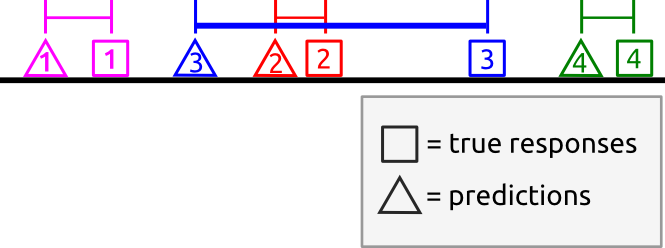
\includegraphics[scale = 0.3]{../../diagram/idloss2a.png} &
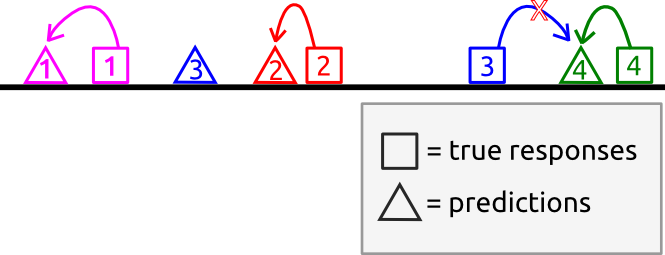
\includegraphics[scale = 0.3]{../../diagram/idloss2b.png} \\
\end{tabular}
\caption{Mean-squared error (a) versus identification accuracy (b) for
  evaluting a multivariate predictive model.}
\label{fig:mse_vs_ia}
\end{figure}

However, an alternative criterion for evaluting the multivariate
linear model was proposed by \cite{Kay2008a}.  In an
\emph{identification task}\cite{Kay2008a}, as illustrated in Figure
\ref{fig:mse_vs_ia}(b), the model is first used to make predictions
\[
\hat{y}_i = B^T \vec{x}_i
\]
for all features $\{\vec{x}_i\}_{i=1}^M$ in the test set Next, each of the
observations $\vec{y}_i$ in the test set is \emph{assigned} to the
closest prediction $\{\hat{y}_j\}_{j=1}^M$ within the test set.
Here, `closest' is defined in terms of the 
the empirical Mahalanobis distance.
\[
d_{\hat{\Sigma}}(\vec{y}, \hat{y}) = (\vec{y} - \hat{y})^T \hat{\Sigma}^{-1} (\vec{y}-\hat{y})
\]
Finally, the $M$-point test identification accuracy is defined as the fraction
of observations which are assigned to the correct prediction,
\[
\text{TIA}_M = \frac{1}{M}\sum_{i=1}^M I(d_{\hat{\Sigma}}(\vec{y}_i, \hat{y}_i) \leq \min_{j \neq i} d_{\hat{\Sigma}}(\vec{y}_i, \hat{y}_i)).
\]

\subsubsection{Advantages of identification accuracy over MSE}

A major reason why identification accuracy was adopted for fMRI
studies is because it provides an intuitive demonstration of how much
information about the stimulus $\vec{X}$ is contained in the response
$\vec{Y}$, in a way that mean-squared error cannot.  We formalize this
idea by explicitly showing how the empirical identification accuracy
can be used to obtain a lower bound of mutual information (Chapter 4).
However, some of the intuition can be demonstrated much more simply
via a toy example.

Suppose that the response $\vec{Y}$ and predictor $\vec{X}$ are both
three-dimensional.  The predictor $\vec{X}$ is generated from a standard
multivariate normal distribution, and then $\vec{Y}$ is generated
according to the linear model
\[
\vec{Y} = B^T \vec{X} + \epsilon
\]
where $\epsilon$ is multivariate normal
\[
\epsilon \sim N(0, \sigma^2 I).
\]

Now consider two different scenarios.  In scenario 1, we have
the model 
\[
\vec{Y}^{(1)} = B^{(1)T} \vec{X} + \epsilon
\]
with
\[
B^{(1)} = \begin{pmatrix}
1 & 1 & 1\\
0 & 0 & 0\\
0 & 0 & 0
\end{pmatrix}
\]
That is, the responses $\vec{Y}$ are only related to the \emph{first}
component of $\vec{X}$.  There is no information in $\vec{Y}$ abut the
other two components of $\vec{X}$, since $\vec{Y}$ is independent of
$(X_2, X_3)$.

In scenario 2, we have the model
\[
\vec{Y}^{(2)} = B^{(2)T} \vec{X} + \epsilon
\]
with
\[
B^{(2)} = \begin{pmatrix}
1 & 0 & 0\\
0 & 1 & 0\\
0 & 0 & 1
\end{pmatrix}
\]
Unlike in scenario 1, now each component $Y_i$ contains information
about a different component $X_i$ of $\vec{X}$.  Therefore, $\vec{Y}$
contains information about all components of $\vec{X}$,

Assume that a large amount of training data is available, so that
there is practically no estimation error for $\hat{B}$.  Suppose the
test set consists of eight points, $(\vec{x}_i, \vec{y}_i)_{i=1}^8$,
where

\[
\begin{matrix}
\vec{x}_1 = (-1, -1, -1) &
\vec{x}_5 = (+1, -1, -1) \\
\vec{x}_2 = (-1, -1, +1) &
\vec{x}_6 = (+1, -1, +1) \\
\vec{x}_3 = (-1, +1, -1) &
\vec{x}_7 = (+1, +1, -1) \\
\vec{x}_4 = (-1, +1, +1) & 
\vec{x}_8 = (+1, +1, +1) \\
\end{matrix}
\]

Let us compare the two scenarios in terms of what happens when we
evaluate the model using mean-squared error.  In both cases, the
mean-squared error will be approximately $3\sigma^2$.  Therefore, MSE
does not distinguish between a low-information situation (Scenario 1)
and a high-information situation (Scenario 2).  Furthermore, since the
expected squared norm of $Y$ is the same in both cases, the
multivariate $R^2$ similarly fails to distinguish the two scenarios.

Now consider the identification accuracy.  In scenario 1, the fact
that $\vec{Y}$ only contains information about $X_1$ means that it can
only separate the two sets $\{\vec{x}_1,\hdots, \vec{x}_4\}$ and
$\{\vec{x}_5,\hdots, \vec{x}_8\}$ from each other, but it cannot
discriminate between stimuli $\vec{x}, \vec{x}'$ which have the same
first component.  It follows that regardless of how small $\sigma^2$
is--even in the noiseless case, the identification accuracy can be at
most $\frac{1}{4}$.  On the other hand, in scenario 2, it is clear
that as $\sigma^2$ goes to zero, that the accuracy increases to 1.  In
figure [] we have computed the identification accuracy for the two
scenarios as a function of $\sigma^2$.


\subsubsection{Cross-validated identification accuracy}



\subsection{Information Theory}\label{sec:intro_mi}

%% Sudden transition

Information theory is motivated by the question of how to design a
message-transmission system, which includes two users--a sender and a
reciever, a \emph{channel} that the sender can use in order to
communicate to the reciever, and a protocol that specifies:
\begin{itemize}
\item[a.] how the sender can \emph{encode} the message in order to
  transmit it over the channel.  Morse code is one example of an
  encoding scheme: a means of translating plaintext into signals than
  can be transmitted over a wire (dots and dashes); and
\item[b.] how the reciever can \emph{decode} the signals recieved from
  the channel output in order to (probabilistically) recover the
  original message.
\end{itemize}

Beginning with Shannon (1948), one constrains the properties of the
channel, and studies properties of encoding/decoding protocols to be
used with the channel.  Two types of channels are studied:
\emph{noiseless} channels, which transmit symbols from a fixed
alphabet (e.g. ``dots'' and ``dashes'') from the sender to reciever,
and \emph{noisy} channels, which transmit symbols from a discrete
symbol space $\mathcal{Y}$ to a possibly different symbol space
$\mathcal{X}$ in a stochastic fashion.  That is, for each input symbol
$y \in \mathcal{Y}$, the transmitted symbol output $X$ is drawn from a
distribution $F_y$ that depends on $y$\footnote{Note that here we
  have flipped the usual convention in information theory, in which
  the letter $X$ commonly denotes the input and $Y$ denotes the
  output.  However, we flip the notation in order to match the
  convention in multi-class classification.}.  It is the study of
noisy channels that is of primary interest to us.

We allow the sender to transmit a sequence of $L$ input symbols over
the channel, $\vec{Y} = (Y_1,Y_2,\hdots, Y_L)$. The reciever will observe the
output $\vec{X} = (X_1,X_2,\hdots, X_L)$, where each $X_i$ is drawn from
$F_{Y_i}$ independently of the previous $X_1,\hdots, X_{i-1}$.

An example of a noisy channel is the \emph{bit-flip} channel.
Let $\mathcal{Y} = \mathcal{X} = \{0,1\}$, so that both the input and output are binary strings.
The bit flip channel is given by
\[
F_0 = \text{Bernoulli}(\epsilon)
\]
\[
F_1 = \text{Bernoulli}(1-\epsilon)
\]
so that $X = Y$ with probability $1-\epsilon$, and $X = 1-Y$
otherwise.

Now, let us assume that the sender wants to transmit message $M$, out
of a finite set of possible messages $\mathcal{M} = \{1,\hdots, m\}$.
The message must be encoded into a signal $\vec{Y} \in \mathcal{Y}^L$,
which is sent through a stochastic channel $F$.  Thus, the encoding
scheme is given by a \emph{codebook} or \emph{encoding function} $g:
\{1,\hdots, m\} \to \mathcal{Y}^L$ which specifies how each message
$i$ is mapped to an input sequence, $g(i) \in \mathcal{Y}^L$.
Conversely, the decoding scheme is given by a decoding function
$d(\vec{X})$ which infers the message $\{1,\hdots, m\}$ from the
recieved signal $\vec{X}$.  Theoretically
speaking\footnote{Practically speaking, the maximum likelihood (ML)
  decoder may be intractable to implement, and computational
  considerations mean that development of practical decoders remains a
  challenging problem.}, a reasonable decoding scheme is the
\emph{maximum likelihood decoder},
\[
d(\vec{x}) = \max_{i \in \{1,\hdots, m\}} \Pr[\vec{X} = \vec{x}| \vec{Y} = g(i)] = \max_{i \in \{1,\hdots, m\}} \prod_{j=1}^L F_{(g(i))_j}(X_j).
\]

The design of encoding/decoding schemes with minimal error (or other
desirable properties) over a fixed channel is a highly nontrivial
problem, which remains a core problem in the information theory
literature.  However, Shannon's original proof of the noisy channel
capacity theorem demonstrates a surprising fact, which is that for
large message spaces $\mathcal{M}$, close-to-optimal information
transmission can be achieved by using a \emph{randomized} codebook.
In order to discuss the noisy channel capacity theorem and the
construction of the randomized codebook, we first need to define
the concept of \emph{mutual information}.

\subsubsection{Mutual information}

If $\bX$ and $\bY$ have joint density $p(\bx, \by)$ with respect to
the product measure $\mu_x \times \mu_y$, then the mutual information
is defined as
\[
\text{I}(\bX;\bY) = \int p(\bx, \by) \log \frac{p(\bx, \by)}{p(\bx)p(\by)}d\mu_x(\bx) d\mu_y(\by).
\]
where $p(\bx)$ and $p(\by)$ are the marginal densities with respect to
$\mu_x$ and $\mu_y$\footnote{Note that the mutual information is
  invariant with respect to change-of-measure.}.  When the reference
measure $\mu_x \times \mu_y$ is unambiguous, note that $\text{I}(\bX;\bY)$ is
simply a functional of the joint density $p(\bx, \by)$.  Therefore, we
can also use the \emph{functional} notation
\[
\text{I}[p(\bx, \by)] = \int p(\bx, \by) \log \frac{p(\bx, \by)}{p(\bx)p(\by)}d\mu_x(\bx) d\mu_y(\by).
\]


The mutual information is a measure of dependence between random
vectors $\bX$ and $\bY$, and satisfies a number of important
properties.
\begin{enumerate}
\item The channel input $\bX$ and output $\bY$ can be random vectors of arbitrary dimension, and the mutual information remains a scalar functional of the joint distribution $P$ of $(\bX, \bY)$.
\item When $\bX$ and $\bY$ are independent, $\text{I}(\bX; \bY) = 0$; otherwise, $\text{I}(\bX; \bY) > 0$.
\item The data-processing inequality: for any vector-valued function $\vec{f}$ of the output space,
\[
\text{I}(\bX; \vec{f}(\bY)) \leq \text{I}(\bX; \bY).
\]
\item Symmetry: $\text{I}(\bX; \bY) = \text{I}(\bY; \bX)$.
\item Independent additivity: if $(\bX_1,\bY_1)$ is independent of $(\bX_2, \bY_2)$, then
\[
\text{I}((\bX_1,\bY_1); (\bX_2, \bY_2)) = \text{I}(\bX_1; \bY_1) + \text{I}(\bX_2; \bY_2).
\]
\end{enumerate}
Three additional consequences result from the data-processing inequality:
\begin{itemize}
\item \emph{Stochastic data-processing inequality}  If $\vec{f}$ is a stochastic function independent of both $\bX$ and $\bY$, then
\[
\text{I}(\bX; \vec{f}(\bY)) \leq \text{I}(\bX; \bY).
\]
This can be shown as follows: any stochastic function $\vec{f}(\bY)$
can be expressed as a deterministic function $\vec{g}(\bY, W)$, where
$W$ is a random variable independent of $\bX$ and $\bY$.
By independent additivity,
\[
\text{I}(\bX; \bY) = \text{I}(\bX; (\bY, W)).
\]
Then, by the data-processing inequality,
\[
\text{I}(\bX; \bY) = \text{I}(\bX; (\bY, W)) \geq \text{I}(\bX; \vec{g}(\bY, W)) = \text{I}(\bX; \vec{f}(\bY)).
\]
\item \emph{Invariance under bijections.} If $\vec{f}$ has an inverse $\vec{f}^{-1}$, then 
\[
\text{I}(\bX; \vec{f}(\bY)) \leq \text{I}(\bX; \bY) = \text{I}(\bX; \vec{f}^{-1}(\vec{f}(\bY))) \leq \text{I}(\bX; \vec{f}(\bY)),
\]
therefore, $\text{I}(\bX; \vec{f}(\bY)) = \text{I}(\bX; \bY)$.
\item \emph{Monotonicity with respect to inclusion of outputs.}  Suppose we have an output ensemble $(\bY_1,\bY_2)$.  Then the individual component $\bY_1$ can be obtained as a projection of the ensemble.  By the data-processing inequality, we therefore have
\[
\text{I}(\bX; \bY_1) \leq \text{I}(\bX; (\bY_1, \bY_2)).
\]
Intuitively, if we observe both $\bY_1$ and $\bY_2$, this can
only \emph{increase} the information we have about $\bX$ compared to
the case where we only observe $\bY_1$ by itself.
\end{itemize}
And it is the property of \emph{invariance under bijections},
inclusive of non-linear bijections, which qualifies mutual information
as a \emph{non-linear measure of dependence.}  Linear correlations are
invariant under scaling and translation, but not invariant
to \emph{nonlinear} bijections.

%As for
%the completeness of the five listed properties: as we know, Shannon's
%mutual information (up to arbitrary scaling factor) is the only
%functional proposed in the literature which satisfies all five
%properties.
Besides the formal definition, there are a number of well-known alternative
characterizations of mutual information in terms of other
information-theoretic quantities: the \emph{entropy} $\text{H}$:
\[
\text{H}_\mu(\bX) = -\int p(\bX) \log p(\bX) d\mu(\bX),
\]
and the \emph{conditional entropy}:
\[
\text{H}_\mu(\bX|\bY) = -\int p(\bY) d\mu_y(\bY) \int p(\bX|\bY) \log p(\bX|\bY) d\mu_x(\bX).
\]
Some care needs to be taken with entropy and conditional entropy since
they are not invariant with respect to change-of-measure: hence the
use of the subscript in the notation $\text{H}_\mu$.  In particular,
there is a difference between \emph{discrete entropy} (when $\mu$ is
the counting measure) and \emph{differential entropy} (when $\mu$ is
$p$-dimensional Lesbegue measure.)  Intutively, entropy measures an
observer's uncertainty of the random variable $\bX$, supposing the
observer has no prior information other than the distribution of
$\bX$. Conditional entropy measures the \emph{expected uncertainty} of
$\bX$ supposing the observer observes $\bY$.

The following identities characterize mutual information in terms of entropy:
\[
\text{I}(\bX; \bY) = \text{H}_{\mu_x \times \mu_y}((\bX, \bY)) - \text{H}_{\mu_x}(\bX) - \text{H}_{\mu_y}(\bY).
\]
\begin{equation}\label{eq:ce_ident}
\text{I}(\bX; \bY) = \text{H}_\mu(\bY) - \text{H}_\mu(\bY|\bX).
\end{equation}
The second identity \eqref{eq:ce_ident} is noteworthy
as being practically important for estimation of mutual information.
Since the entropies in question only depend on the marginal and
conditional distributions of $\bY$, the problem of estimating
$\text{I}(\bX; \bY)$ can be reduced from a $\dim(\bX)
+ \dim(\bY)$-dimensional nonparametric estimation problem to a
$\dim(\bY)$-dimensional problem: hence this identity is a basis of
several methods of estimation used in neuroscience, such as Gastpar
(2014).

However, by symmetry, we also have the flipped identity
\begin{equation}\label{eq:ce_ident2}
\text{I}(\bX; \bY) = \text{H}_\mu(\bX) - \text{H}_\mu(\bX|\bY).
\end{equation}
Loosely speaking, $\text{H}_\mu(\bX)$ is the uncertainty of $\bX$
before having observed $\bY$, and $\text{H}_\mu(\bX|\bY)$ is the
uncertainty of $\bX$ after having observed $\bY$, hence
$\text{H}_\mu(\bX) - \text{H}_\mu(\bX|\bY)$ is how much the
observation of $\bY$ has \emph{reduced} the uncertainty of $\bX$.
Stated in words,
\[
\text{I}(\bX; \bY) = \text{average reduction of uncertainty about $\bX$ upon observing $\bY$}.
\]

\subsubsection{Channel capacity and randomized codebooks}

As a general measure of dependence, mutual information has enjoyed
numerous and diverse applications outside of information theory.
However, its original role in Shannon's paper was to define the
quantity known as \emph{channel capacity} of a noisy channel.

Let us first note that the channel capacity of a noiseless channel
with $S$ symbols is simply $\log S$.  The justification is that if we
allow $L$ symbols to be sent, then $S^L$ possible messages can be
encoded.  Therefore, the channel capacity of a noiseless channel can
be understood as the logarithm of the number of possible messages to
be transmitted divided by the length of the sequence, with is $\log
S$.

However, how can the idea of channel capacity be generalized to the
noisy case?  At first glance, it would seem like no comparison is
possible, because no matter how many symbols $L$ the sender is allowed
to transmit, it may \emph{never} be possible for the reciever to
deterministically infer the original message.  Consider the bit-flip
channel, where $X = Y$ with probability $1-\epsilon$ and $X = 1-Y$
otherwise.  Given two different messages, $M \in \{1,2\}$, a
reasonable encoding scheme is for the sender to transmit a string of
$L$ repeated zeros for $M = 1$, and an string of $L$ repeated ones for
$M = 2$.
\[
Y_1 = Y_2 = \cdots = Y_L = M-1.
\]
The reciever should guess $M = 1$ if she recieves more zeros than
ones, and guess $M = 2$ otherwise.  However, for any $L$, the decoding
error will always be nonzero.  Therefore there seems to be no analogy
to the noiseless channel, where zero decoding error can be achieved.

Shannon's idea was to invent an asymptotic definition of channel
capacity.  Consider a sequence of problems where the number of
messages $M$ is increasing to infinity.  In the $m$th coding problem,
where $M = m$, let $(g_m, d_m)$ be an encoder/decoder pair (or \emph{protocol}), where
$g_m$ produces strings of length $L_m$.  Let $e_m$ be the maximimum
error probability over all messages $1,\hdots, m$ when using the
protocol $(g_m, d_m)$.  Now, let us require that we choose $(g_m,
d_m)$ so that the error probability vanishes in the limit:
\[
\lim_{m \to \infty} e_m \to 0.
\]
We can define the channel capacity to be the best possible limiting ratio
\[
C = \lim_{m \to \infty} \frac{\log m}{L_m}
\]
over all sequences of protocols that have vanishing error probability.
Note that this definition yields $C = \log S$ for the noiseless
channel, but can also be extended to the noisy channel case.
Remarkably, Shannon finds an explicit formula for the noisy channel
capacity, which is proved in his noisy channel capacity theorem.  We
will now discuss how to calculate the capacity of a noisy channel.

First, let us define the set of joint distributions which can be
realized in the noisy channel.  Let $p_y$ be a probability
distribution over input symbols $\mathcal{Y}$.  If we transmit input
$Y$ randomly according to $Y \sim p_y$, the induced joint distribution
$p(Y, X)$ is given by
\[
p(y, x) = p_y(y) F_y(\{x\}).
\]
The set $\mathcal{P}$ is simply the collection of all such distributions: that is,
\[
\mathcal{P} = \{p(y, x) \text{ such that } p(x|y) = F_y(\{x\})\text{ for all }(x, y) \in \mathcal{X} \times \mathcal{Y}\}.
\]

Suppose we have a noisy channel with transmission probabilities given by $\{F_y\}_{y \in \mathcal{Y}}$.
Shannon came with with the following result:
\[
C = \max_{p\in \mathcal{P}} I[p(y, x)].
\]
The noisy channel capacity is given by the maximal mutual information
$I(Y; X)$ over all joint distributions of $(Y, X)$ that can be
realized in the channel.

To show that $C = \max_p I[p(y, x)]$ is the noisy channel capacity,
then, (i) we need to show that there exists a sequence of codes with
length $L = \frac{\log M}{C}$ which achieves vanishing decoding error
as $M \to \infty$\footnote{Shannon's noisy channel capacity theorem
  shows a much stronger property--that the \emph{maximum} decoding
  error over all messages has to vanish.  However, for our purposes,
  we will limit our discussion to a weaker form of the noisy channel
  capacity theorem which is only concerned with average decoding error
  over all messages.}, and (ii) we need to show that any code with a
shorter length has non-vanishing decoding error.  We omit the proof of
(i) and (ii), which can be found in any textbook on information
theory, such as \cite{Cover2006}.  However, for our purposes, it is
very much worth discussing the construction that shows direction (i)
of the proof--the achievability of channel capacity.

For a given channel $\{F_y\}$, let $p^* \in \mathcal{P}$ be the
distribution which maximizes $I[p(y, x)]$.  Let $p^*_y$ be the
marginal distribution of $Y$, and let $L = \lceil \frac{\log M}{C}
\rceil$.  Now we can define the random code.  Let $g(i) =
(Y_1^{(i)},\hdots, Y_L^{(i)})$ where $Y_j^{(i)}$ are iid draws from
$p^*_y$ for $i = 1,\hdots, M$ and $j = 1,\hdots, L$.  Shannon proved
that average decoding error, taken over the distribution of random
codebooks, goes to zero as $M \to \infty$.  This implies the existence
of a deterministic sequence of codebooks with the same property, hence
establishing (i).


\subsection{Comparisons}

We see that in both the multi-class classification problem and the
noisy channel model present examples of discrimination problems where
one must recover some latent variable $Y$ from observations $X$, where
$X$ is related to $Y$ through the family of conditional distributions
$F_Y$.  One difference is that while in multi-class classification,
$F_Y$ is unknown and has to be inferred from data, in the noisy
channel model, the stochastic properties of the channel $F_Y$ are
usually assumed to be known.  A second difference is that in the noisy
channel model, there is a choice in how to specify the encoding
function $g(M)$, which affects subsequent performance.  Finally, in
the broader research context, machine learning research has
traditionally focused on multi-class problems with relatively few
classes, while information theory tends to consider problems in
asymptotic regimes where the number of possible messages $m$ is taken
to infinity. These differences were sufficient to explain why little
overlap exists in the respective literatures between multi-class
classification and the noisy channel model.

%% unusual to put mention this here

However, an interesting development in the machine learning community
has been the application of multi-class classification to problems
with increasingly large and complex label sets.  Consider the
following timeline of representative papers in the multi-class
classification literature:
\begin{itemize}
\item Fisher's Iris data set, \cite{fisher1936use}, $K = 3$ classes
\item Letter recognition, \cite{frey1991letter}, $K = 26$ classes
\item Michalski's soybean dataset, \cite{mickalstd1980learning}, $K = 15$ classes
\item The NIST handwritten digits data set, \cite{grother1995nist}, $K = 10$ classes
\item Phoneme recognition on the TIMIT datset, \cite{clarkson1999use}, $K = 39$ classes
\item Object categorization using Corel images, \cite{duygulu2002object} $K = 371$ classes
\item Object categorization for ImageNet dataset, \cite{deng2010does}, $K = 10,184$ classes
\item The 2nd Kaggle large-scale hierarchical text classification challenge (LSHTC), \cite{partalas2015lshtc}, $K = 325,056$
\end{itemize}
As we can see, in recent times we begin to see classification problems
with extremely large label sets.  In such large-scale classification
problems, or `extreme' classification problems, results for $K \to
\infty$ numbers of classes, like those found in information theory,
begin to look more applicable.

This work focuses on a particular intersection between multi-class
classification and information theory, which is the study of
\emph{random classification tasks.}  In numerous domains of applied
mathematics, it has been found that systems with large numbers of
components can be modelled using randomized versions of those same
systems, which are more tractable to mathematical analysis: for
example, studying the properties of networks by studying random graphs
in graph theory, or studying the performance of combinatorial
optimization algorithms for random problem instances.  Similarly, it
makes sense to posit randomized models of multi-class discrimination
problems.  Since information theorists were the first to study
discrimination problems with large number of classes, we find in the
information theory literature a long tradition of the study of
\emph{random code} models.  This thesis is dedicated to the the study
of the analogue of random code models in the multi-class
classification setting: models of \emph{randomized classification,}
which we motivate and analyze in the next chapter.

%% Make the connection between random codes and randomized classification,
%% point out why randomized classification is a good model for some contemporary problems


%% Link back to Shannon and information theory.  We develop further links between randomized classification and information theory.

%% omit this section 

\iffalse

\section{Neuroscience applications}

Both supervised learning and information theory are routinely used as
tools in the study of human and animal brains.  While Shannon's theory
of information was motivated by the problem of designing
communications system, the applicability of mutual information was
quickly recognized by neuroscientists.  Only four years after
Shannon's seminal paper in information theory (1948), McKay and
McCullough (1952) inaugurated the application of mutual information to
neuroscience. Since then, mutual information has enjoyed a celebrated
position in both experimental and theoretical neuroscience.

Supervised learning also has an extensive history of interaction with
neuroscience.  Notably, the development of artificial neural networks
in supervised learning was motivated by models of biological neural
networks.  Examining the hierarchical nature of the visual system
inspired the development of convolutional neural networks [CITE].
More recently, neuroscientists have begun to explore the possibility
of using supervised learning models to model brain functionality.
This approach is especially valuable for the problem of understanding
specialization in the brain.

We now illustrate these use cases of information theory and supervised
learning in a number of specific applications in neuroscience.

\subsection{Selecting decoding models.}\label{sec:model_selection}
Neurons carry information via \emph{spike trains}, which are temporal
point processes.  In response to stimulus $\bX$, the neuron produces a
spike train $Y(t)$ where $Y(t) = 1$ indicates a spike at time $t$ and
$Y(t) = 0$ indicates no spiking, for $t \in [0, T]$.

An open question in neuroscience that of how information is encoded in
the spike train.  Put loosely, what is `signal' in the spike train
$Y(t)$ and what is `noise'?  Presumably there exists
some \emph{decoder}--some function $\vec{g}$ of the time series, which
compresses $Y(t)$ to a small dimension while preserving most of the
information about $\bX$.

Nelken et. al. (2005) investigated the neural code in the A1 auditory
cortex of a cat, in response to recorded birdsongs.  The stimulus $\bX
= (X_1, X_2)$ takes the form of 15 different auditory recordings
presented in 24 spatial directions: $X_1 \in \{1,\hdots, 15\}$ indexes
the recording and $X_2 \in \{1,\hdots, 24\}$ indexes the direction of
presentation.  The response $Y(t)$ takes the form of a spike train.

Nelkin et. al. compare the following \emph{decoders} $\vec{g}$ in terms
of the information $\text{I}(\bX; \vec{g}(Y(t)))$.
\begin{itemize}
\item The total spike count $\vec{g}_1(Y(t)) = \sum_t Y(t)$.
\item The mean response time $\vec{g}_2(Y(t)) = \frac{1}{\sum_t Y(t)} \sum_t t Y(t)$.
\item The combination of the two codes: $\vec{g}_{1+2}(Y(t)) = (\vec{g}_1(Y(t)), \vec{g}_2(Y(t)))$.
\end{itemize}
The information of each decoder is compared to the full information of
the signal, $\text{I}(\bX; Y(t))$, which is estimated via binning.

Nelkin et al. find that while the decoder $\vec{g}_1$ reduces the
mutual information by 20 to 90 percent, the information loss from
$\vec{g}_2$ is much less, and barely any information at all is lost
when both decoders are used jointly in $\vec{g}_{1+2}$.  The
scientific conclusion that can be drawn is that since
$\text{I}(\bX; \vec{g}_{1+2}(Y(t)))$ is not much smaller than
$\text{I}(\bX; Y(t))$, the ``signal'' in the spike train is mostly
captured by the spike counts and response times: beyond that, the
detailed temporal pattern of spiking is likely to be ``noise.''  Of
course, an important caveat to their conclusions is
only \emph{individual} neurons are considered: the analysis did not
rule out the possibility that the temporal spiking pattern could yield
information within an \emph{ensemble} of neurons.

\subsection{Inferring functional specialization}\label{sec:searchlight}

Historically, the earliest discoveries
of specialized modules in the brain were due to lesion studies, where
patients who had parts of their brain destroyed due to injury or
clinical surgeries also lost cognitive or motor functionality as a
result.  The loss of functionality established a causal pathway
between the lesioned area and the affected behavior--as, for example,
in the case of the discovery of Broca's area, which was established in
this way to be critical for speech production [CITE].  However,
ethical and practical limitations restrict the use of lesioning as an
experimental technique, and furthermore, lesion studies cannot be
applied to exhaustively isolate the regions of the brain which are
specialized for a given task.

Therefore, an alternative method of studying specialization is to
acquire an image of the brain activity, and then to assess the
discriminative performance of classifiers on either the whole brain,
the brain minus a number of ``lesioned'' areas, or isolated regions of
the brain by themselves.  The classifier may achieve a certain
accuracy using the whole brain image, and reduced accuracies using
``lesioned'' images--and, given the removal of the task-critical parts
of the brain in the image, may be reduced to chance accuracy levels.
Therefore, similar to lesion studies, these classification experiments
can reveal specialization in the brain by establishing which parts of
the brain image contain \emph{information} related to the task.  This
type of classification study was first introduced to the neuroimaging
community by Haxby (1999); approaches of these types are known as
\emph{multivariate pattern analyses} (MVPA) in the neuroscience
literature. However, an important distinction between MVPA studies and
actual lesion studies is that MVP analyses can only establish
association, rather than causality, because actual lesions to the
brain affect the activity patterns of other parts of the brain, and
therefore the effect of lesions cannot actually be completely
simulated by merely masking parts of the brain image.
%% examples where the artificial classifier does mimic the natural classifier

\subsubsection{Data Setup}

While multivariate pattern analysis can be applied in a wide variety
of brain imaging modalities, its dominant use has been in functional
magnetic resonance imaging (fMRI.)  Therefore, we will briefly
describe the experimental setup and initial data analysis protocol for
a typical task-fMRI experiment.  For more details, the interested
reader is invited to consult a standard reference such as
\cite{poldrack2011handbook}.

In task-fMRI experiments, a subject is presented with a timed sequence
of behaviorial tasks to be performed, while the MRI scanner uses
magnetic fields to measure blood oxygenation levels in the subject's
brain.  The raw imaging data is obtained in Fourier space.  Initial
preprocessing converts the data into a spatial time series consisting
of one time dimension and three spatial dimensions, with measure of
BOLD (blood-oxygenation level dependent) signal at each point in the
brain.  Further preprocessing steps reduce noise due to head motion,
physiologically induced artifacts, and electromagnetically induced
artifacts.  A generalized linear model (GLM) is fitted to the spatial
time series in order to infer an aggregated activity level for each
specific task.  We do not go into details of the GLM model; however,
the output of the GLM model is an inferred activity level map for each
task.

Figure \ref{fig:task_fmri} illustrates a cartooon schematic of the
output of the GLM fitting stage.  There are four tasks in the
illustrated experiment.  Each task $y_i$ belongs to two different
categories, coded as 1 and 2.  Task 1 is a visual task, where the
subject is presented an picture of an eagle, and asked to focus on the
image.  Task 2 is the same type of visual task, but with a picture of
a bear instead.  For each task $i=1,\hdots, 4$, the GLM produces a
parametric map of inferred activation levels, $\vec{x}_i$.  The map
$\vec{x}_i$ is divided into uniformly sized cubical regions in the
brain, called \emph{voxels}.  We denote the number of voxels in the
map by $q$; for typical resolutions ($2\text{mm} \times 2 \text{mm}
\times 2.5 \text{mm}$), the map has on the order of $q = 20,000$
voxels.  Each voxel has an inferred activity level.  Therefore, the
map $\vec{x}_i$, when represented as a numerical vector, is a vector
in $\mathbb{R}^q$ where each component is the activity level of a
particular voxel in the brain.


\begin{figure}
\centering
\begin{tabular}{|c|cc|c|}
\hline
Task & Stimulus & & Activation Map\\ \hline
1 & $y_1 = 1$ & 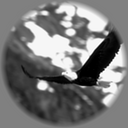
\includegraphics[scale = 0.26]{../../proposal/img3.png} & $\vec{x}_1 = $ 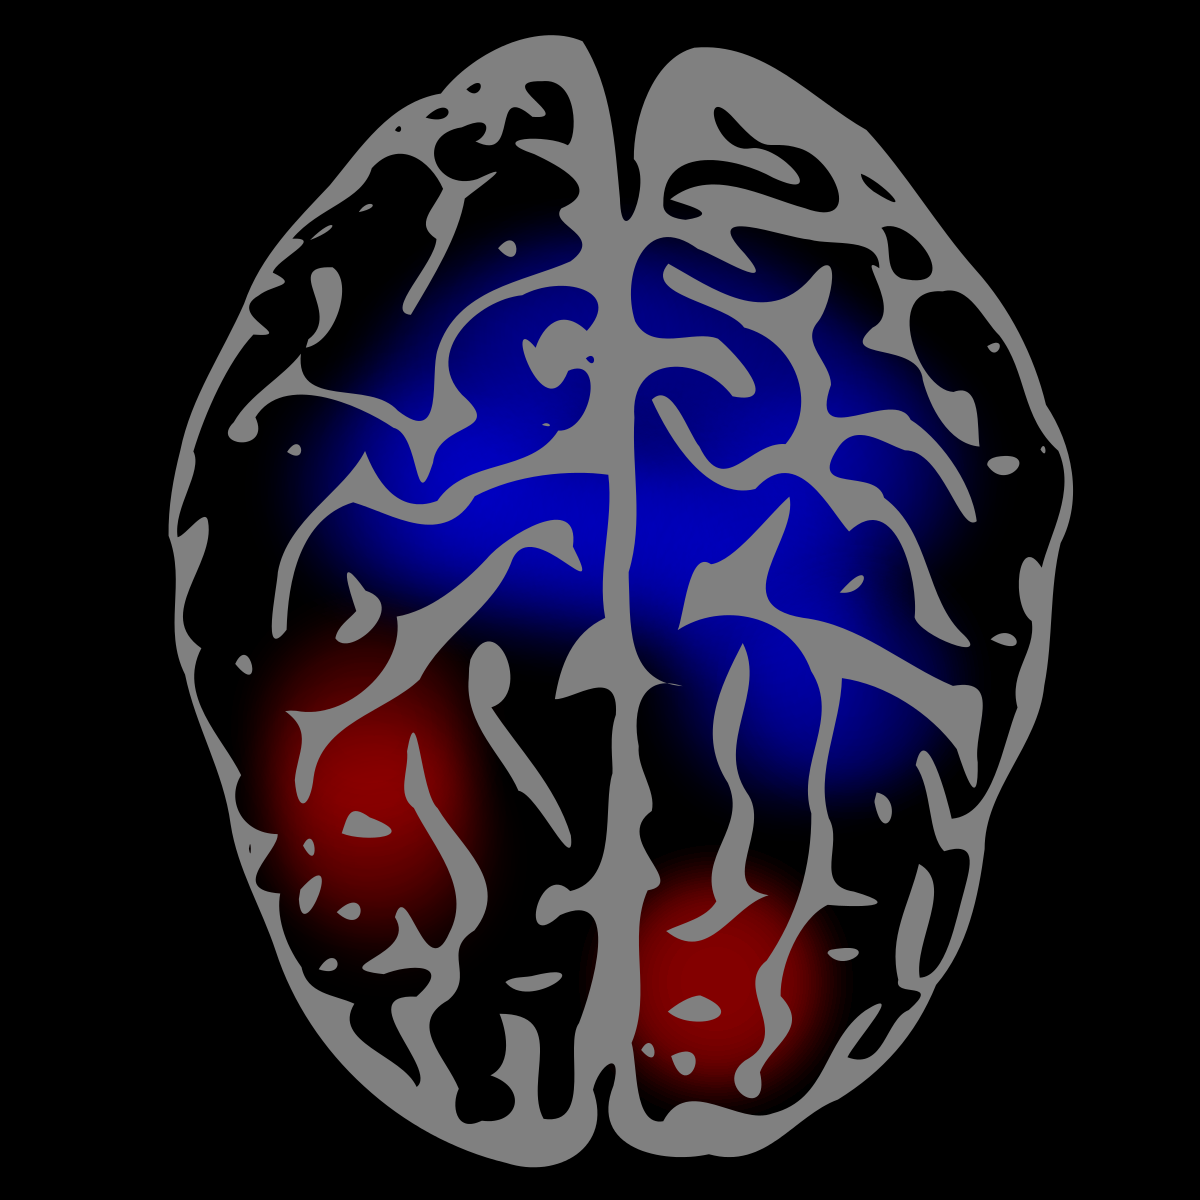
\includegraphics[scale = 0.035]{../../proposal/brain1.png} \\ \hline
2 & $y_2 = 2$ & 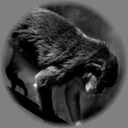
\includegraphics[scale = 0.26]{../../proposal/img4.png} & $\vec{x}_2 = $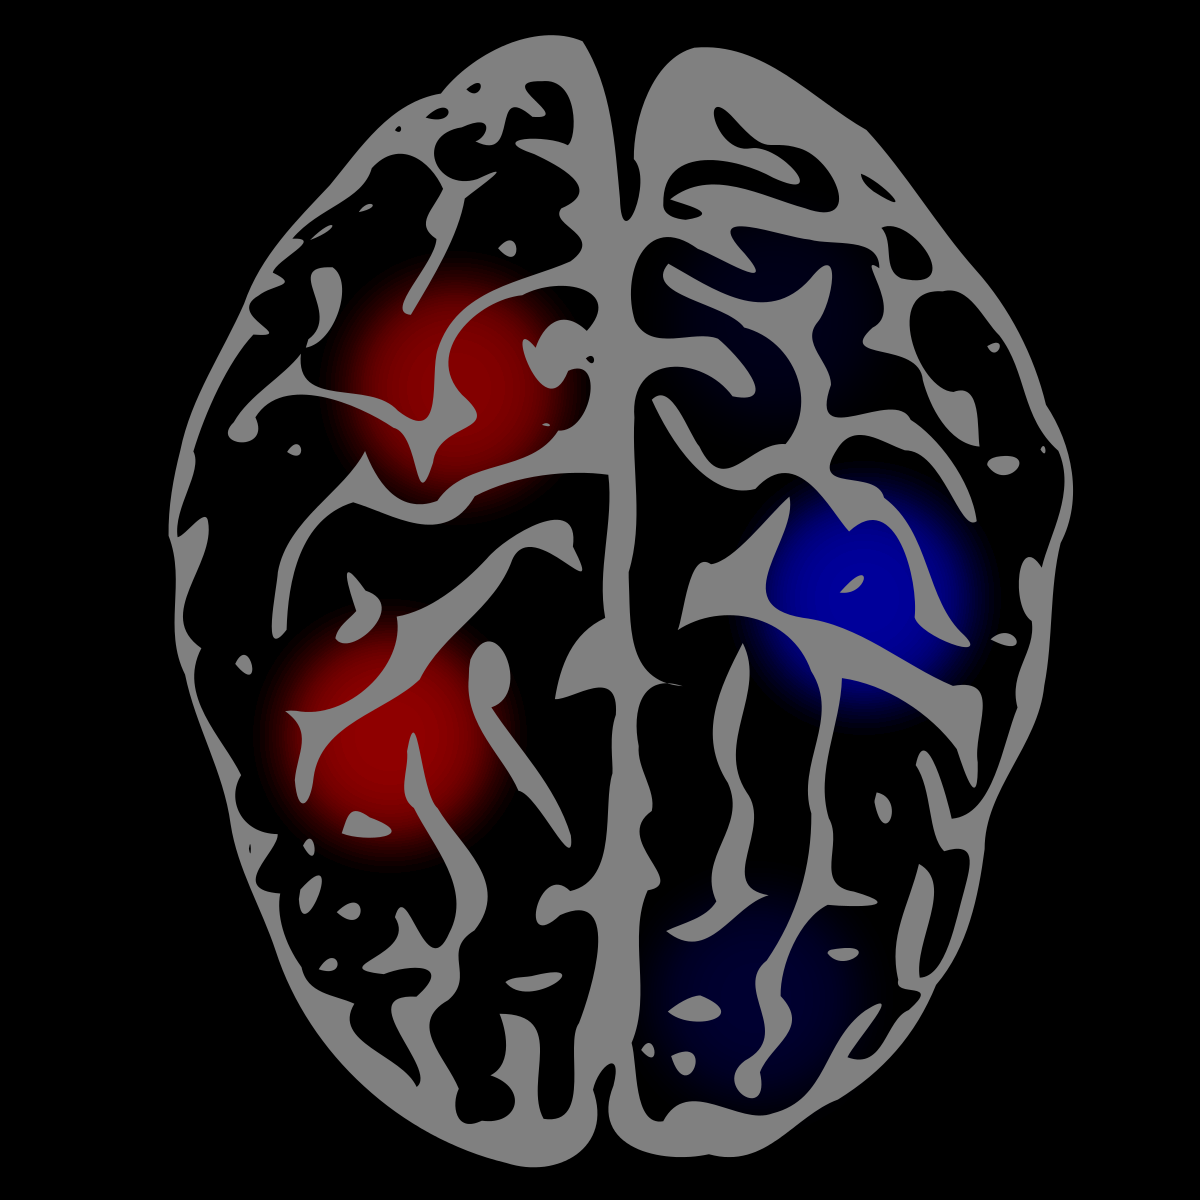
\includegraphics[scale = 0.035]{../../proposal/brain3.png} \\ \hline
3 & $y_3 = 1$ & 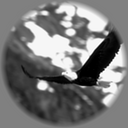
\includegraphics[scale = 0.26]{../../proposal/img3.png} & $\vec{x}_3 = $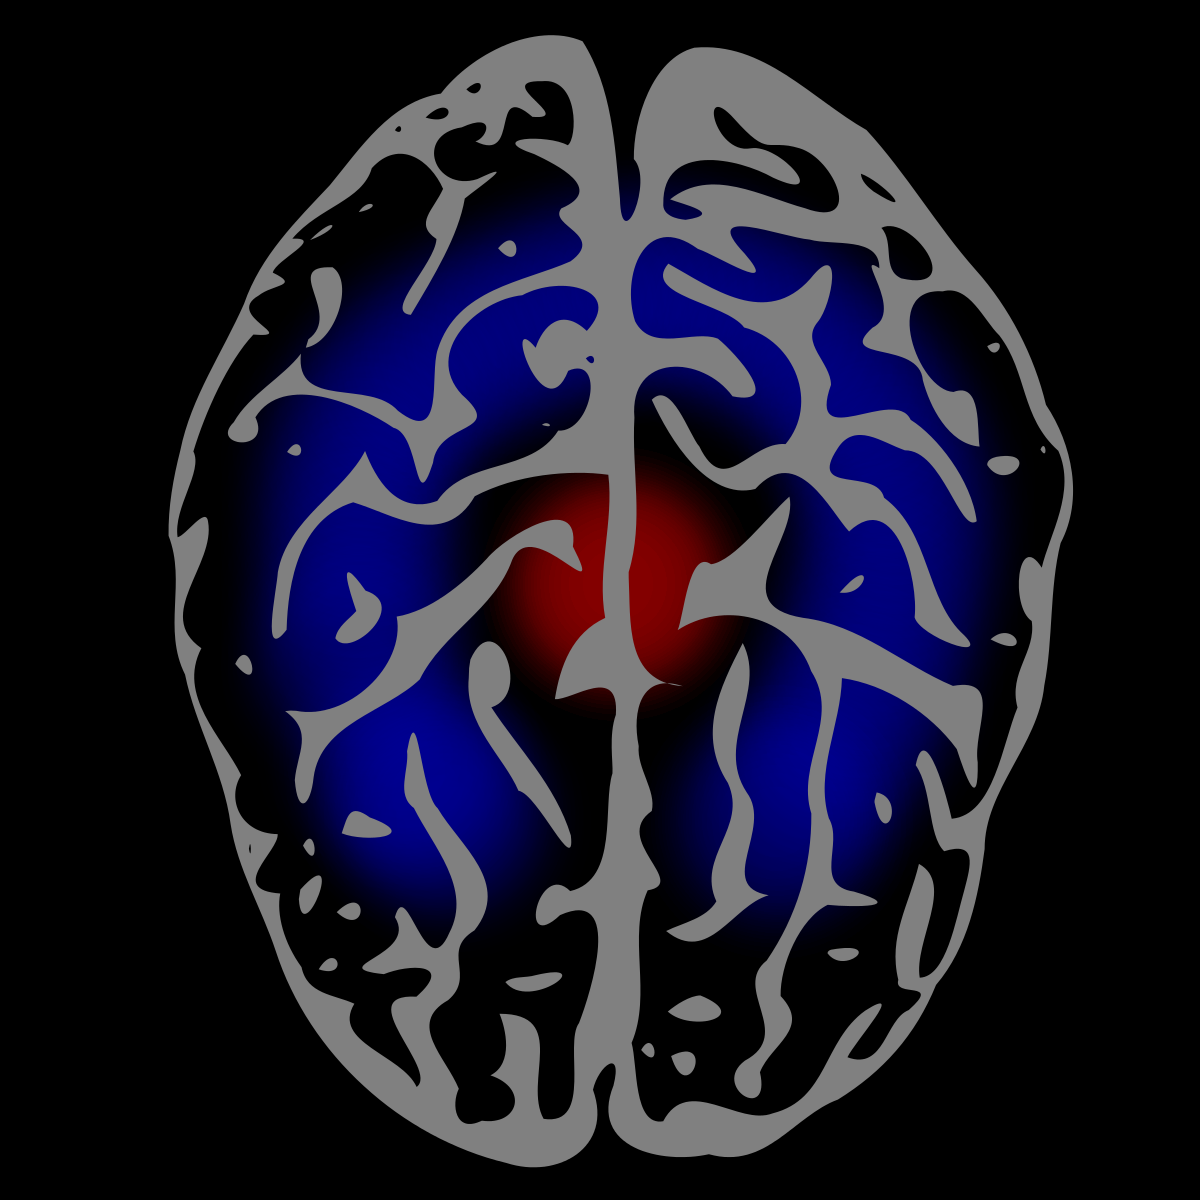
\includegraphics[scale = 0.035]{../../proposal/brain4.png} \\ \hline
4 & $y_4 = 2$ & 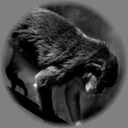
\includegraphics[scale = 0.26]{../../proposal/img4.png} & $\vec{x}_4 = $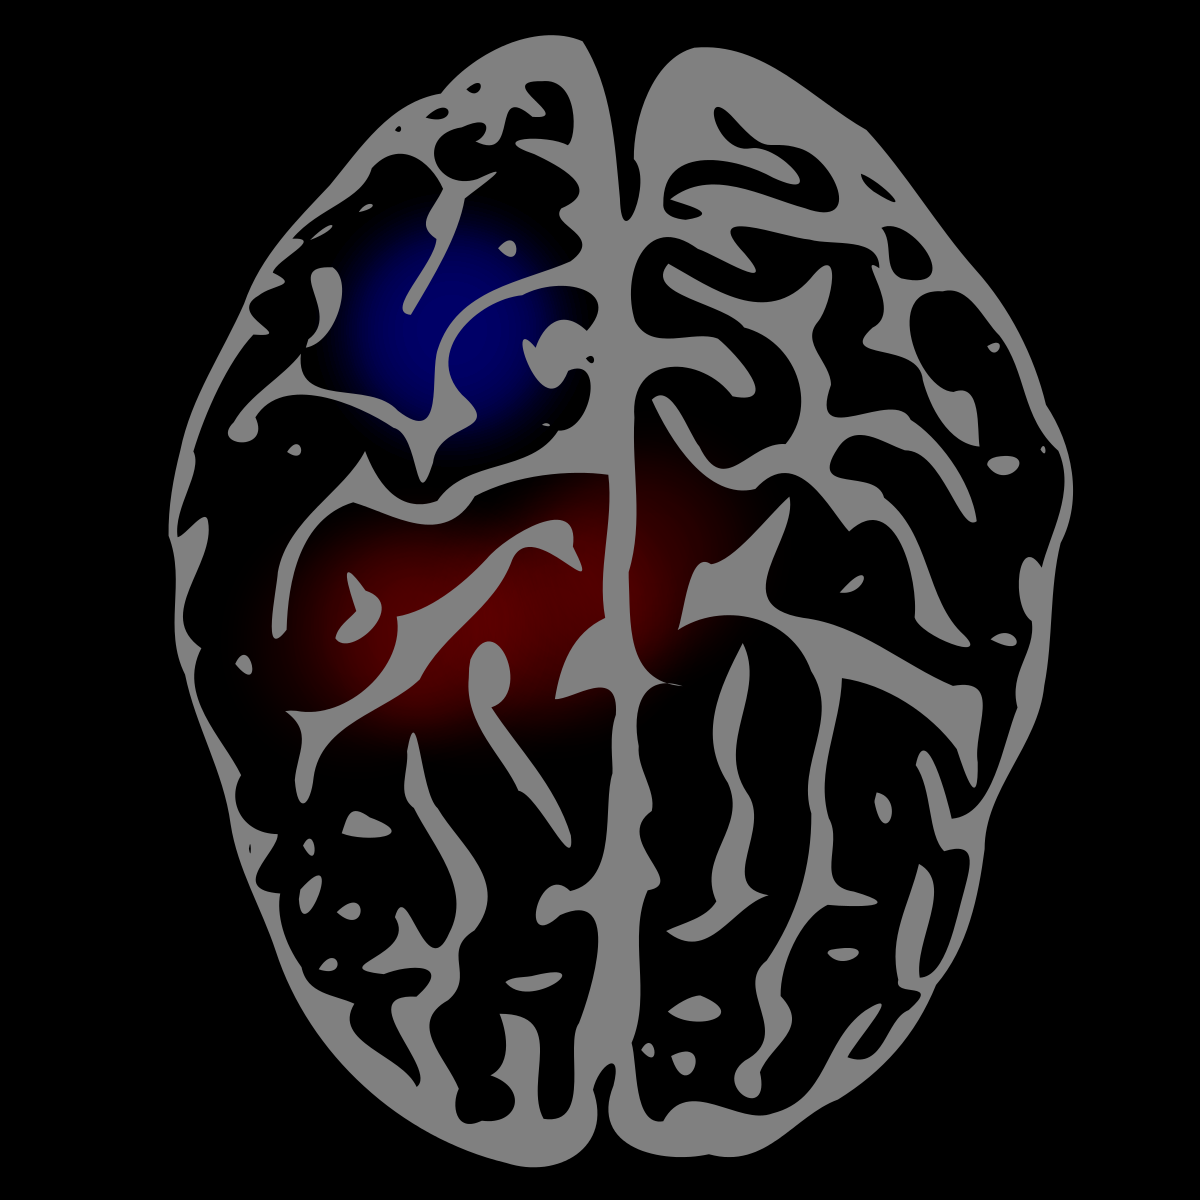
\includegraphics[scale = 0.035]{../../proposal/brain8.png} \\ \hline
\end{tabular}
\caption{Data output of a typical analysis of a task fMRI experiment.
  The raw data is processed to obtain a parametric map of inferred
  activation levels to each stimulus.  These activation levels are
  further utilized in downstream analyses. }
\label{fig:task_fmri}
\end{figure}

A number of statistical analyses can be performed on the
task-activation pairs $(y_i, \vec{x}_i)$.  The most common type of
analysis tests for significant \emph{peaks} of task-correlated
activity.  These analyses involve \emph{global} tests of the null
hypothesis of no correlation between task and activity.  However, MVPA
analyses tend to begin with local tests of independence between a
given region-of-interest (a cluster of neighboring voxels) and the
task.

\subsubsection{Classification-based test of independence}

A region of interest (ROI) is a collection of neighboring voxels,
chosen based on anatomical or geometric considerations.  To give a
concrete example, one can choose an arbitrary voxel in the brain, and
define an ROI as the set of all voxels within a given radius (say, $5
\text{mm}$) of the chosen voxel.  Recalling that $\vec{x}_i$ denotes
the activity level of the entire brain, let us write $\vec{x}_i^{ROI}$
for the subset of voxels in the brain map belonging to the ROI.

We would like to test the hypothesis of independence between the task
$Y$ and the joint activity level of the voxels belonging to the ROI,
considered as a random vector, $\vec{X}^{ROI}$.  While there are
numerous methods in the statistical literature for testing for
independence between a categorical random variable $Y$ and a random
vector $\vec{X}$, the approach taken in MVPA is typically to use
classification accuracies as the test statistic.

Recall that a classification rule is any (possibly stochastic) mapping
$f: \mathcal{X} \to \{1,\hdots, k\}$, where $k$ is the number of
levels of $Y$.  Let us assume that the $k$ different levels of $Y$
have the same number of repeats within the data.  The
\emph{generalization accuracy} of the classification rule is
\[
\text{GA}(f) = \frac{1}{k} \sum_{i=1}^k\Pr[f(\vec{X}^{ROI}) = i | Y = i].
\]
A trivial classification rule which outputs the result of a $k$-sided
die roll for all inputs $y$ would achieve a generalization accuracy of
$\text{GA} = \frac{1}{k}$.

Recall that the generalization accuracy of a data-dependent
classification rule $f$ can be obtained by using
\emph{data-splitting}, provided that the rule $f$ is constructed using
only the \emph{training data}.  Supposing that the original data
consists of pairs $(y_i,\vec{x}_i^{ROI})$ for $i = 1,\hdots, n$, let
$j_1,\hdots, j_{n_1}$ denote the $n_1$ randomly drawn training
indices, and $\ell_1,\hdots, \ell_{n_2}$ denote the $n_2$ randomly
drawn test indices.  The training data $(y_{j_i},
\vec{x}_{j_i}^{ROI})_{i=1}^{n_1}$ is used to construct a classification rule
$f$, while the test data is used to obtain a test accuracy $T$:
\[
T= \frac{1}{n_2} \sum_{i=1}^{n_2} I(f(\vec{x}_{\ell_i}^{ROI}) = y_{\ell_i}).
\]
%% also give the formula for stratifying by class

Under the null hypothesis $H_0: Y \perp \vec{X}^{ROI}$, the
generalization accuracy of any classification rule $f$ is equal to
$1/k$.  Therefore, we can write the null hypothesis as
\[
H_0: \text{GA}(f) = \frac{1}{k}
\]
and the alternative hypothesis as
\[
H_1: \text{GA}(f) > \frac{1}{k}.
\]

We will describe two different methods for testing $H_0$ versus $H_1$.
The first approach is to use the fact that the distribution of $T$ is
known under the null hypothesis.  The second approach is a permutation
test\footnote{Permutation tests are
widely used in statistical applications: for a good introduction to
the subject, the reader is invited to consult
\cite{efron1994introduction}.}.  The permutation test is more computationally expensive, but has
important advantages in terms of family-wise error control, as we will
describe in the sequel. %% describe in the next subsubsection

\emph{First approach.} Under the null hypothesis, using the fact that
the test observations $(y_{\ell_i}, \vec{x}_{\ell_i})$ are identical
and independently distributed from the population distribution of
stimulus-activity pairs, we have
\[
n_2 T \sim_{H_0} \text{Bernoulli}(n_2, \frac{1}{k})
\]
Therefore, let $c_\alpha$ be the $(1-\alpha)$ quantile of a
$\text{Bernoulli}(n_2, \frac{1}{k})$ distribution.  To perform a
hypothesis test at level $\alpha$, reject the null $H_0$ if $n_2 T >
c_\alpha$ and accept otherwise.  Equivalently, define the $p$-value as
the area under the tail of the $\text{Bernoulli}(n_2,
\frac{1}{k})$ distribution to the right of $T$,
\[
p = \Pr[X > n_2 T| X \sim \text{Bernoulli}(n_2, \frac{1}{k})],
\]
and reject if and only if $p < \alpha$.

\emph{Second approach (permutation test)}.  Under the null hypothesis of
independence between $Y$ and $\vec{X}^{ROI}$, the test statistic $T$
(the test accuracy on $n_2$ test observations) has a distribution that
is invariant under permutation of the labels $Y_1,\hdots, Y_n$.
Therefore, obtain $B$ samples of permutation test statistics
$T^{(1)},\hdots, T^{(B)}$ by the following procedure:
\begin{itemize}
\item[1.] For $j = 1,\hdots, B$, draw a random permutation $\sigma: n \to n$.
\item[2.] Use the pairs
  $(y_{\sigma_i},\vec{x}^{ROI}_{\sigma_i})_{i=1}^{n_1}$ to construct
  classification rule $f^{(j)}$ (using the same classifier as the one
  used to construct $f$).
\item[3.] Evaluate the test accuracy of $f^{(j)}$,
\[
T^{(j)}= \frac{1}{n_2} \sum_{i=1}^{n_2} I(f^{(j)}(\vec{x}_{\sigma_i}^{ROI}) = y_{\sigma_i}).
\]
\end{itemize}
The permutation $p$-value is calculated based on the rank of $T$ within the sample of permuation test statistics:
\[
p = \frac{\sum_{j=1}^B I(T^{(j)} < T) + 1}{B + 1},
\]
and reject the null hypothesis if and only if $p < \alpha$.

\subsubsection{Searchlight analysis}

Classifier-based tests of independence are commonly combined with the
\emph{multivariate searchlight} procedure
(\cite{kriegeskorte2006information}, \cite{kriegeskorte2007analyzing})
in order the scan the entire brain for informative clusters of voxels.
The procedure produces a 3D map of $p$-values in the brain, with
significant $p$-values indicative of regions in the brain associated
with the task.  Figure \ref{fig:searchlight_example} displays one
example of a $p$-value map obtained from an object perception task (\cite{chen2011cortical}).

\begin{figure}
\centering
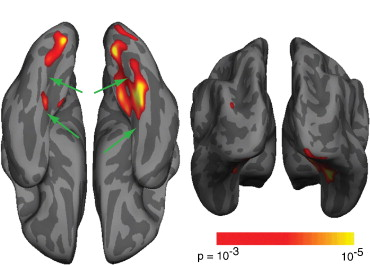
\includegraphics[scale = 0.5]{Figures/chen2010_cropped.png}
\caption{$p$-value map obtained from linear SVM-based searchlight
  applied to object perception data, using spherical neighborhoods
  with 9mm radius (\cite{chen2011cortical}).}
\label{fig:searchlight_example}
\end{figure}

A \emph{searchlight} refers to a local region-of-interest centered
around a particular \emph{central voxel}.  A variety of methods can be
used to define the neighborhood.  The most straightforward is the
\emph{spherical searchlight}, which fixes a radius $r$, and to include
all voxels within a distance $r$ of the central voxel.  However, more
sophisticated approaches may account for the geometry of the brain
surface (\cite{chen2011cortical}.)

Having chosen a method for obtaining searchlights, one generates a
searchlight centered around each voxel in the fMRI image, $\vec{x}$.
Let $\{ROI_1,\hdots, ROI_v\}$ denote the collection of such
searchlights, with $\vec{X}^{ROI_i}$ consisting of the voxels centered
around the $i$th voxel.

For each $ROI_i$, one conducts a hypothesis test for independence
between $Y$ and $\vec{X}^{ROI_i}$ using the local test of independence
described earlier.  % in the previous subsection This produces a map
of $p$-values, $p_1,\hdots, p_v$, for each voxel in the fMRI image.
Clusters of small $p$-values can be informally interpreted as
indicative of brain regions associated with the task.  Alternatively,
to test the global null hypothesis that all ROIs are independent of
the task, one can apply the permutation testing approach
simultaneously to all voxels in the brain.  The global permuation
approach is carried out as follows:
\begin{itemize}
\item[0.] (Non-permuted data): Draw a random permutation $\sigma: n \to n$. For $i = 1,\hdots, v$, use the pairs
  $(y_{\sigma_\ell},\vec{x}^{ROI_i}_{\sigma_\ell})_{\ell=1}^{n_1}$ to construct
  classification rule $f^{(0, i)}$
\item[1.] For $j = 1,\hdots, B$, draw a random permutation $\sigma: n \to n$.
\item[2.] For $i = 1,\hdots, v$, use the pairs
  $(y_{\sigma_\ell},\vec{x}^{ROI_i}_{\sigma_k})_{\ell=1}^{n_1}$ to construct
  classification rule $f^{(j, i)}$ (using the same classifier as the one
  used to construct $f$).
\item[3.] Evaluate the test accuracy $T^{(j,i)}$ of $f^{(j, i)}$.
\item[4.] Find the maximum accuracy $T^{(j)} = \max_{i=1}^v T^{(j,i)}$.
\item[5.] Define the $p$-value for each ROI by
\[
p_i =  \frac{\sum_{j=1}^B I(T^{(j)} < T^{(0, i)}) + 1}{B + 1},
\]
\end{itemize}
Since the permutations are shared across the ROIs, familywise control
is attained, in the sense that $p^* = \min_i p_i$ is a valid
$p$-value.

\subsection{Other applications of mutual information}

Experimentally, mutual information has been used to detect strong
dependencies between stimulus features and features derived from
neural recordings, which can be used to draw conclusions about the
kinds of stimuli that a neural subsystem is designed to detect, or to
distinguish between signal and noise in the neural output.
Theoretically, the assumption that neural systems maximize mutual
information between salient features of the stimulus and neural output
has allowed scientists to predict neural codes from signal processing
models: for instance, the center-surround structure of human retinal
neurons matches theoretical constructions for the optimal filter based
on correlations found in natural images [cite].

\subsection{Can classification accuracy quantify information?}

Due to the analogy between the nervous system and a communications
network, it was a natural choice for early neuroscientists to adopt
Shannon's \emph{mutual information} as a quantitative measure of
dependence, as we saw in the application of mutual information to
decoding models (Section \ref{sec:model_selection}).  But as new
technologies enabled the recording of neural data at larger scales and
resolution, the traditional reductionist goals of neuroscience were
supplemented by increasingly ambitious attempts within neuroscience to
understand the dynamics of neural ensembles, and by efforts
originating within psychology and medicine to link the structure and
function of the entire human brain to behavior or disease.  The scale
of the data, and the complexity of the models studied posed an
obstacle to traditional information-theoretic approaches.  Therefore,
it was of considerable interest when Haxby (2001) introduced the usage
of \emph{supervised learning} (classification tasks) for the purpose
of quantifying stimulus information in task fMRI scans, as we
discussed in section \ref{sec:searchlight}.

Judging from the language used by the practioners themselves, it is
intuitively clear to them how classification accuracies can be used to
quantify information in brain scans.  We agree with the intuition
behind this practice, and go further to say that the use of
classification accuracies as a measure of information can be formally
justified.  However, having said this, it is important to remark that
Shannon's \emph{mutual information} need not be taken as the canonical
quantification of ``information'' as a measure of multivariate
dependence.  Instead, we take a step back and attempt to dissect the
intuitive properties of ``information'' and why the concept is useful
in science.  We will argue that given these intuitions, both mutual
information and classification accuracy can be seen as useful measures
of information.

\begin{itemize}
\item \emph{
Intuition 1: Information is a measure of dependence.}   If $\bX$ and $\bY$ are statistically independent, then
$\bX$ gives no information about $\bY$, and vice-versa.
\end{itemize}
This intuition is employed when researchers test the null hypothesis
of chance accuracy for classification.  If the null is accepted, the
researcher concludes that there is no information in the predictors
about the response.

\begin{itemize}
\item \emph{
Intuition 2a: Monotonicity with respect to inclusion of outputs.} If $\bX_1$ and $\bX_2$ are ensembles of neurons (or
individual neurons), then the combined ensemble $(\bX_1, \bX_2)$ has equal or
more information about $\bY$ than either component by itself.
\end{itemize}

\begin{itemize}
\item \emph{
Intuition 2b: Noise adds no information.} If, in the previous example, $\bX_2$ is independent of
$\bY$, then $\bX_2$ adds no information to the ensemble.
\end{itemize}
The non-informativity of noise is vital for the purpose of
\emph{localizing} information within fMRI voxels (as is done in
searchlight analysis.)  Since noise voxels fail to improve
classification performance (and indeed, sometimes harm empirical
performance,) the optimal searchlight radius will concentrate on
clusters of signal voxels, and minimize the inclusion of noise voxels.

\begin{itemize}
\item \emph{Intuition 3:}
Information can be used as a basis of model selection.  Among multiple
encoding/decoding models, a more accurate model should tend to have
greater information relative to less accurate models.  
\end{itemize}
Compared to the first two, this third intuition is somewhat less
obvious, but nevertheless appears as an important use-case for mutual
information, as seen in the application of mutual information to
choose encoding models.

%Arguably, both the application of mutual information described in
%\ref{sec:model_selection} and the use of classification accuracies in
%\ref{sec:searchlight} are justified by this common set of three
%intuitions.

It is well-known that the mutual information $I(\bX; \bY)$ satisfies
these three intuitions.  However, the \emph{Bayes classification
  accuracy}--the accuracy of the \emph{optimal} classifier, also
satifies these three intuitions.  
\begin{enumerate}
\item When $\bX$ and $\bY$ are
independent, then the Bayes accuracy falls to chance, $1/k$,
indicating `no information.'  
\item As additional predictors are made available, the Bayes accuracy
  can only improve.  As noise predictors are addded, the Bayes
  accuracy remains unchanged.
\item Supposing that there exists a `true encoding' with $\bY$ only
  depending on some function basis $\vec{b}(\bX)$, then the Bayes
  accuracy for predicting $\bY$ from the basis $\vec{g}(\bX)$ is
  maximized when $\vec{g} = \vec{b}$.
\end{enumerate}

However, an important caveat is that classification accuracies
attained in practice are at best an \emph{underestimate} of Bayes
accuracy, and therefore do not perfectly inherit all of the above
properties.  For instance, while the Bayes accuracy satisfies
Intuition 2b, classification accuracy generally does not: due to the
phenomenon of overfitting, the inclusion of noise predictors reduces
classification accuracy.

On the other hand, given sufficient training observations and
well-specification of models, classification accuracies begin to
approach Bayes accuracies, and therefore can be justifiable used as
measures of information which satisfy Intuitions 1-3.  This link
between empirical classification accuracies, Bayes accuracies, and
information forms the basis for much of the work in this thesis.

That said, a deeper understanding of the conditions which allow
attained classification accuracies to mimic the properties of Bayes
classification accuracy would be greatly useful for understanding the
practical limitations of some of the methods that will be proposed in
the later chapters.  However, we must leave this important work for
future research.

\fi

